% Ergebnisse - Endergebnisse der Arbeit, Performance, Bilder (auf dpi achten, mind. 300), Kennkurven, Warps, weitere Leistungsmessungen bez. auf meine Arbeit
% -> ggf. Results and Discussion seperat halten
% Bedeutung der Ergebnisse (im Rahmen dessen was wissenschaftlich haltbar ist)
\chapter{Ergebnisse und Diskussion}\label{chap::resdisc}
In den Ergebnissen werden die verschiedenen Raycast Methoden auf Bildqualität und Performanz untersucht.
Anschließend folgt eine Diskussion bezüglich der verschiedenen Ergebnissen.

\section{Ergebnisse}\label{sec::results}
Der erste Abschnitt beinhaltet Ergebnisse der Implementierungen des Standard Raycasts, \emph{MDC} \ref{ss::MDC} und \emph{DDC} \ref{ss::DDC} sowie der Implementierung der Variierung der Strahlabtastrate \ref{sec::workpacks::ors}.
Dabei liegt der Fokus auf die Beschreibung der wahrgenommenen Bildqualität der verschiedenen Methoden.
Der zweite Abschnitt beinhaltet gemessene Performanzleistungen der jeweiligen Implementierungen bei der Verwendung unterschiedlicher Transferfunktionen und Volumendaten.
Die verschiedenen Methoden werden hier im Hinblick auf die benötigten Ausführungszeiten bei Berechnungen mit verschiedenen Volumen verglichen.

\subsection{Bildqualität}
Für die Bildqualität werden Screenshots von Berechnungen mit unterschiedlichen Raycast Methoden vorgestellt, bewertet und verglichen.
Die Bewertung erfolgt anhand der wahrgenommenen Bildqualität und wie diese sich verändert, wenn die Bildabtastrate und die Strahlabtastrate variiert werden.
Es wird von drei Methoden die Bildqualität untersucht, wobei diese jeweils Ergebnisse mit unterschiedlichen Bildabtastraten produzieren.
Diese sind: Standard-, \emph{MDC}- und \emph{DDC}-Methode.
Die Bildqualität dieser Methoden wird einmal mit konstanter Strahlabtastrate und einmal mit variierte Strahlabtastrate vorgestellt.
Dafür werden zwei Volumen verwendet, wobei die Ergebnisse des ersten Volumens für die unterschiedlichen Methoden getrennt-, und die Ergebnisse mit dem zweiten Volumen im Anschluss für einen besseren Vergleich zusammen vorgestellt werden.

Die Ergebnisse in diesem Abschnitt wurden alle mit einer Auflösung von $2263\times1306$\,Pixel berechnet.
Alle Abbildungen, die das selbe Volumen zeigen, wurden mit der gleichen Transferfunktion und aus der gleichen Perspektive berechnet.
Die Unterschiede bei der Berechnung ergeben sich ausschließlich aus einer veränderten Bild- oder Strahlabtastrate.

Der Begriff \emph{maximale Bildabtastrate} bezieht sich auf die Bildabtastrate mit einem Wert von circa $1$ und bedeutet, dass für jeden Pixel des Bildes ein Strahl berechnet wurde, der den Farbwert des Pixels angibt.
Eine Bildabtastrate von $\frac{1}{2}$ bedeutet, dass in x- und y-Richtung nur für jeden zweiten Pixel ein Strahl berechnet wurde.
Eine Bildabtastrate von $\frac{1}{7}$ bedeutet, dass in x- und y-Richtung nur für jeden siebten Pixel ein Strahl berechnet wurde.
Die Bildabtastrate kann theoretisch aber auch auf einen Wert größer als $1,0$ gesetzt werden.
In allen Berechnungen, außer bei der Methode \emph{MDC}, wurde die maximale Bildabtastrate $1,0$ gewählt.
Aufgrund der Implementierung und der verwendeten Auflösung für die Berechnungen ist die Bildabtastrate für die Methode \emph{MDC} nur $0,96$.
Dies wird bei der Bewertung aber wie eine Bildabtastrate von $1,0$ behandelt. 

Die Strahlabtastrate gibt an, in welchem Abstand ein Strahl abgetastet wird.
Die Abtastdistanz wird mit $\frac{1\times Voxellaenge}{maximale Strahlabtastrate}$ berechnet.
Die Voxellänge ergibt sich aus der Skalierung der Voxel, welche abhängig von den verwendeten Volumen ist.
In allen Berechnungen ist die maximale Strahlabtastrate $1,5$ gewählt worden.

Wurde eine Abbildung mit variierter Strahlabtastrate berechnet, so bedeutet dies, dass die Strahlabtastrate an der Mausposition den maximalen Wert der Strahlabtastrate hat.
Mit zunehmender Distanz zur Mausposition nimmt die Strahlabtastrate dann bis auf einen Wert von $\frac{maximale Strahlabtastrate}{4}$ ab.

Das erste Volumen ist ein ct-scan eines Bonsai Baums.
Das Volumen hat eine Auflösung von $256\times256\times256$\,Voxel.
Die Slice-Dicke der einzelnen Voxel ist $1,0\times1,0\times1,0$ und gibt die Skalierung der einzelnen Voxel an.
Das heißt, dass die Voxel in x-, y- und z-Richtung hier eine einheitliche Skalierung haben.

\subsubsection{Standard Raycast}\label{ss::res::sr}
Abbildung \ref{fig::res::bon_st} zeigt eine Berechnung des Volumens \emph{Bonsai} mit dem Standard Raycast.
Die Bildabtastrate ist bei der Berechnung des Standard Raycasts im ganzen Bild homogen und hat den Wert $1$.
Die Strahlabtastrate ist für das ganze Bild konstant und hat den Wert $1,5$.
Das heißt, dass für jeden Pixel des Bildes ein Work-Item gestartet wurde, um den Raycast eines Strahls zu berechnen.
Der jeweilige Pixel erhält die berechnete Farbe des Work-Items.

Durch die Interpolation der Voxel wird das Volumen mit weichen Konturen und Flächen gezeichnet.
Die Transferfunktion hebt die Voxel mit etwas höherer Dichte farblich hervor.
Dadurch sind farblich einheitliche und zusammenhängende Strukturen erkennbar, unter Anderem die Blätter, Äste und den Stamm.
Die Voxel, die nicht zu dem Bonsai Objekt gehören, zum Beispiel Leerräume, haben teilweise auch Dichtewerte größer null.
Daher wurde die Transferfunktion so gewählt, dass diese ebenfalls vollständig ausgeblendet sind.
Insgesamt werden die Flächen aber transparent gezeichnet, so dass auch eigentlich verdeckte Strukturen zu sehen sind.

Wie in den Grundlagen im Abschnitt \ref{sec::eye} zum visuellen Wahrnehmungssystem beschrieben wurde, kann man feststellen, dass wenn ein bestimmter Punkt in der Abbildung \ref{fig::res::bon_st} fokussiert wird, die vom Blickpunkt entfernten Bereiche unscharf erscheinen.
Im Standard Raycast werden auch diese mit normaler Bildabtastrate gezeichnet, obwohl dies aufgrund der Limitierungen des visuellen Wahrnehmungssystems, eigentlich nicht notwendig ist.

In Abbildung \ref{fig::res::bon_st_ors} wurde das Volumen auch mit dem Standard Raycast verwendet aber die Strahlabtastrate variiert.
Mit zunehmender Distanz zur Mausposition, welche als schwarzes Kreuz eingezeichnet wurde, nimmt die Strahlabtastrate ab.
Dies ist selbst an weit von der Mausposition entfernten Objekten, an denen die Strahlabtastrate am niedrigsten ist, kaum wahrnehmbar.
Wird die Mausposition selbst fokussiert, ist kein Unterschied feststellbar.

\begin{landscape}
	\begin{figure}
		\centering
		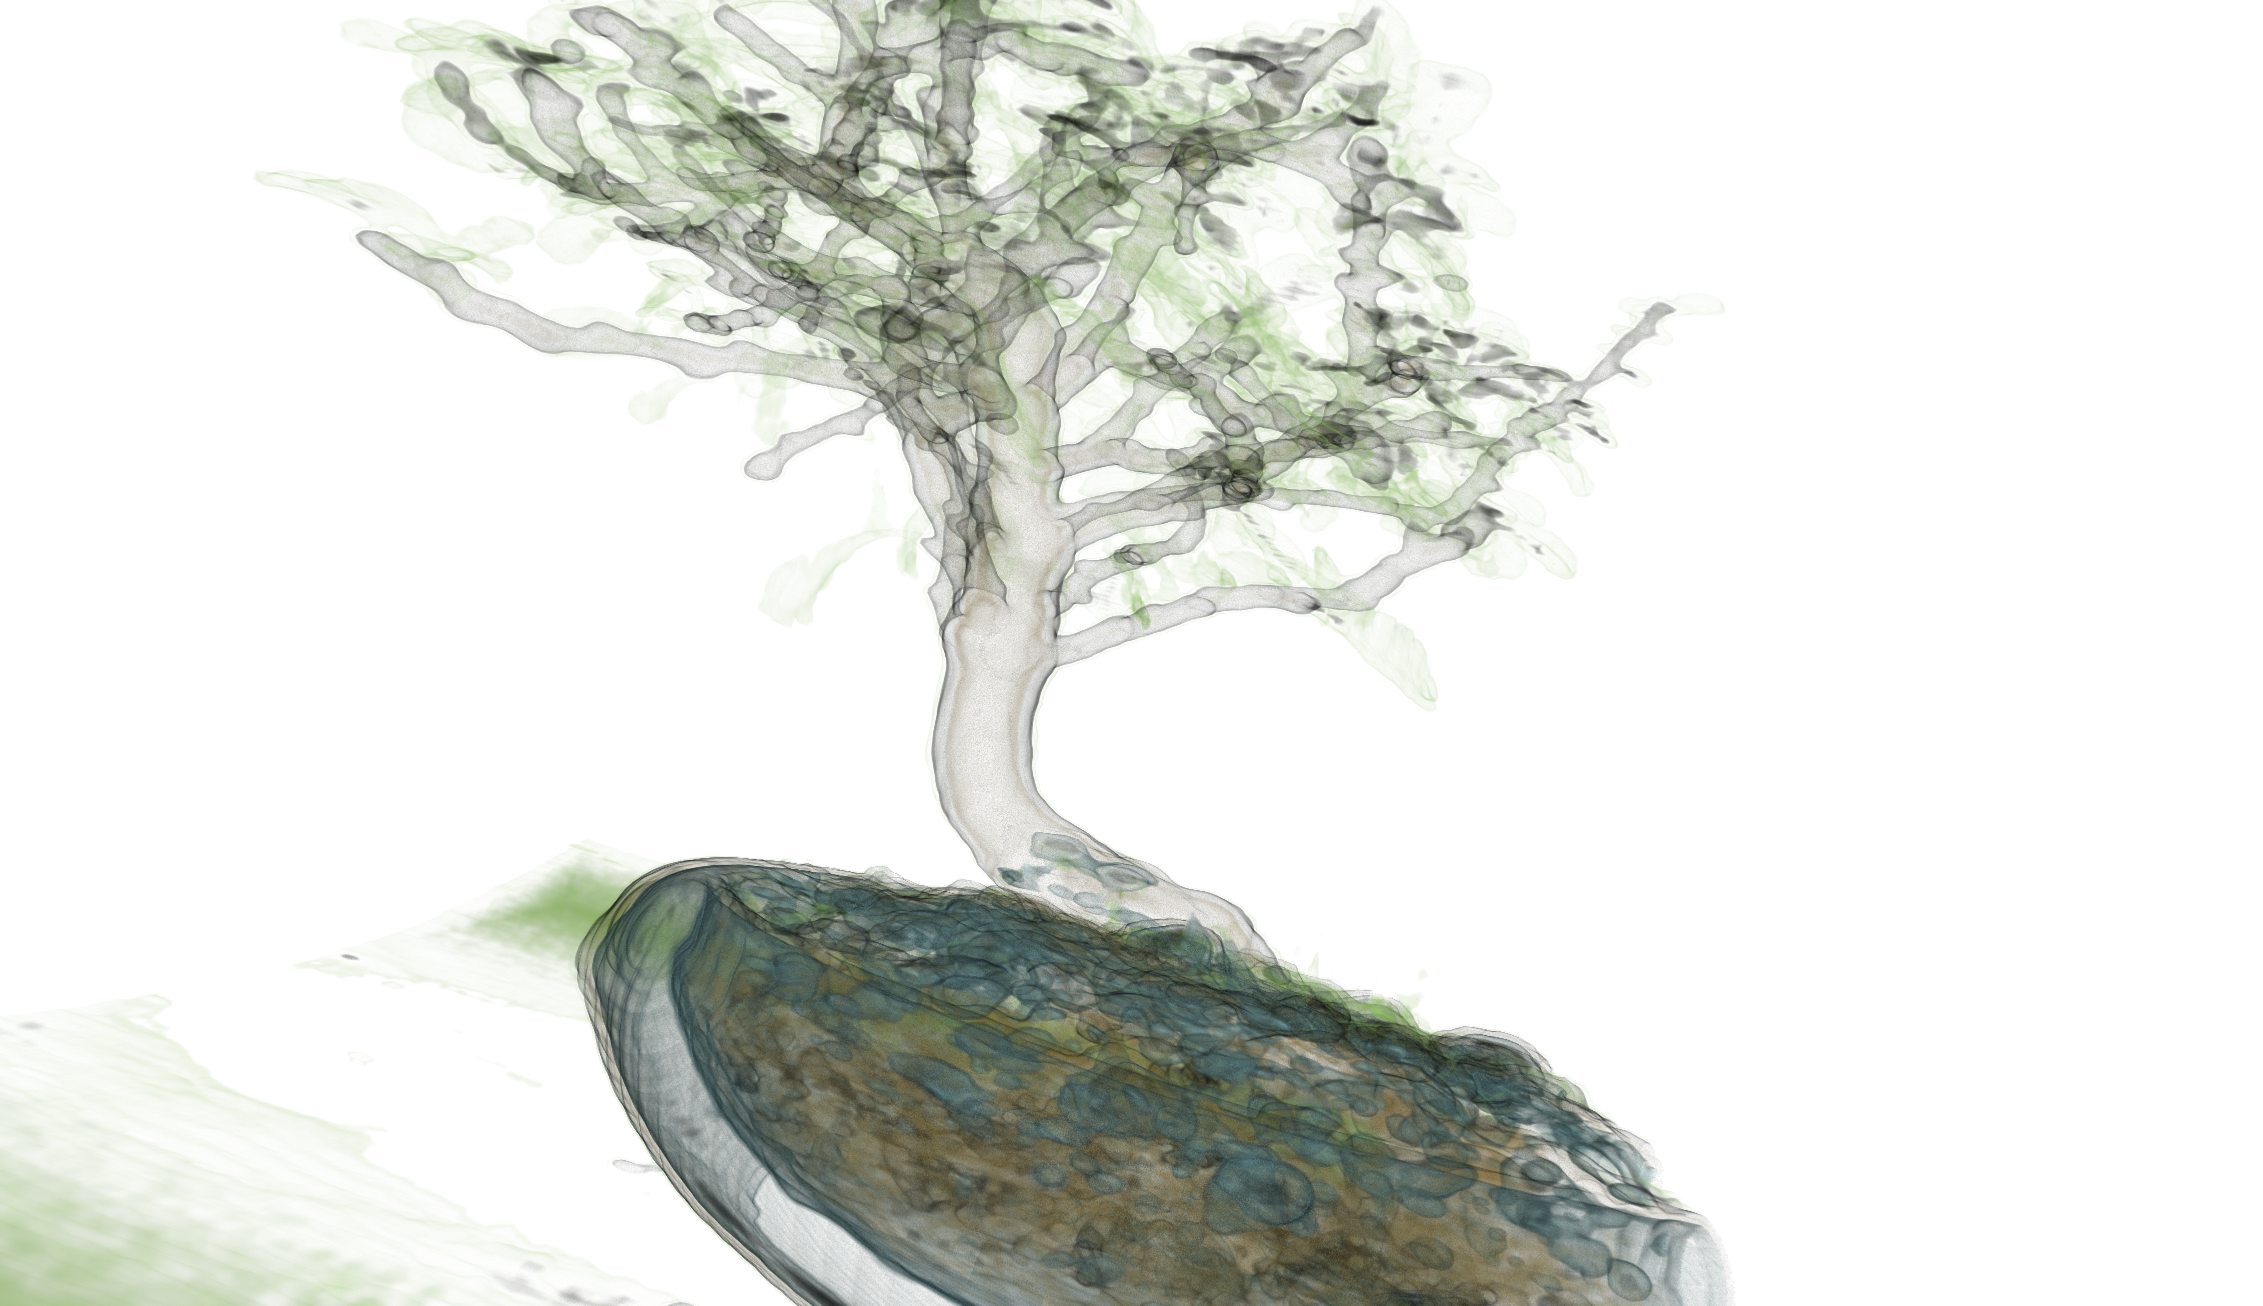
\includegraphics[width=\textheight]{../../Neue_Messungen/Bonsai/st.png}
		\caption{Volumen Bonsai mit ursprünglichem Raycast berechnet. Das Bild hat eine Bildabtastrate von $1$ und eine Strahlabtastrate von $1,5$.}
		\label{fig::res::bon_st}
	\end{figure}
\end{landscape}

\begin{landscape}
	\begin{figure}
		\centering
		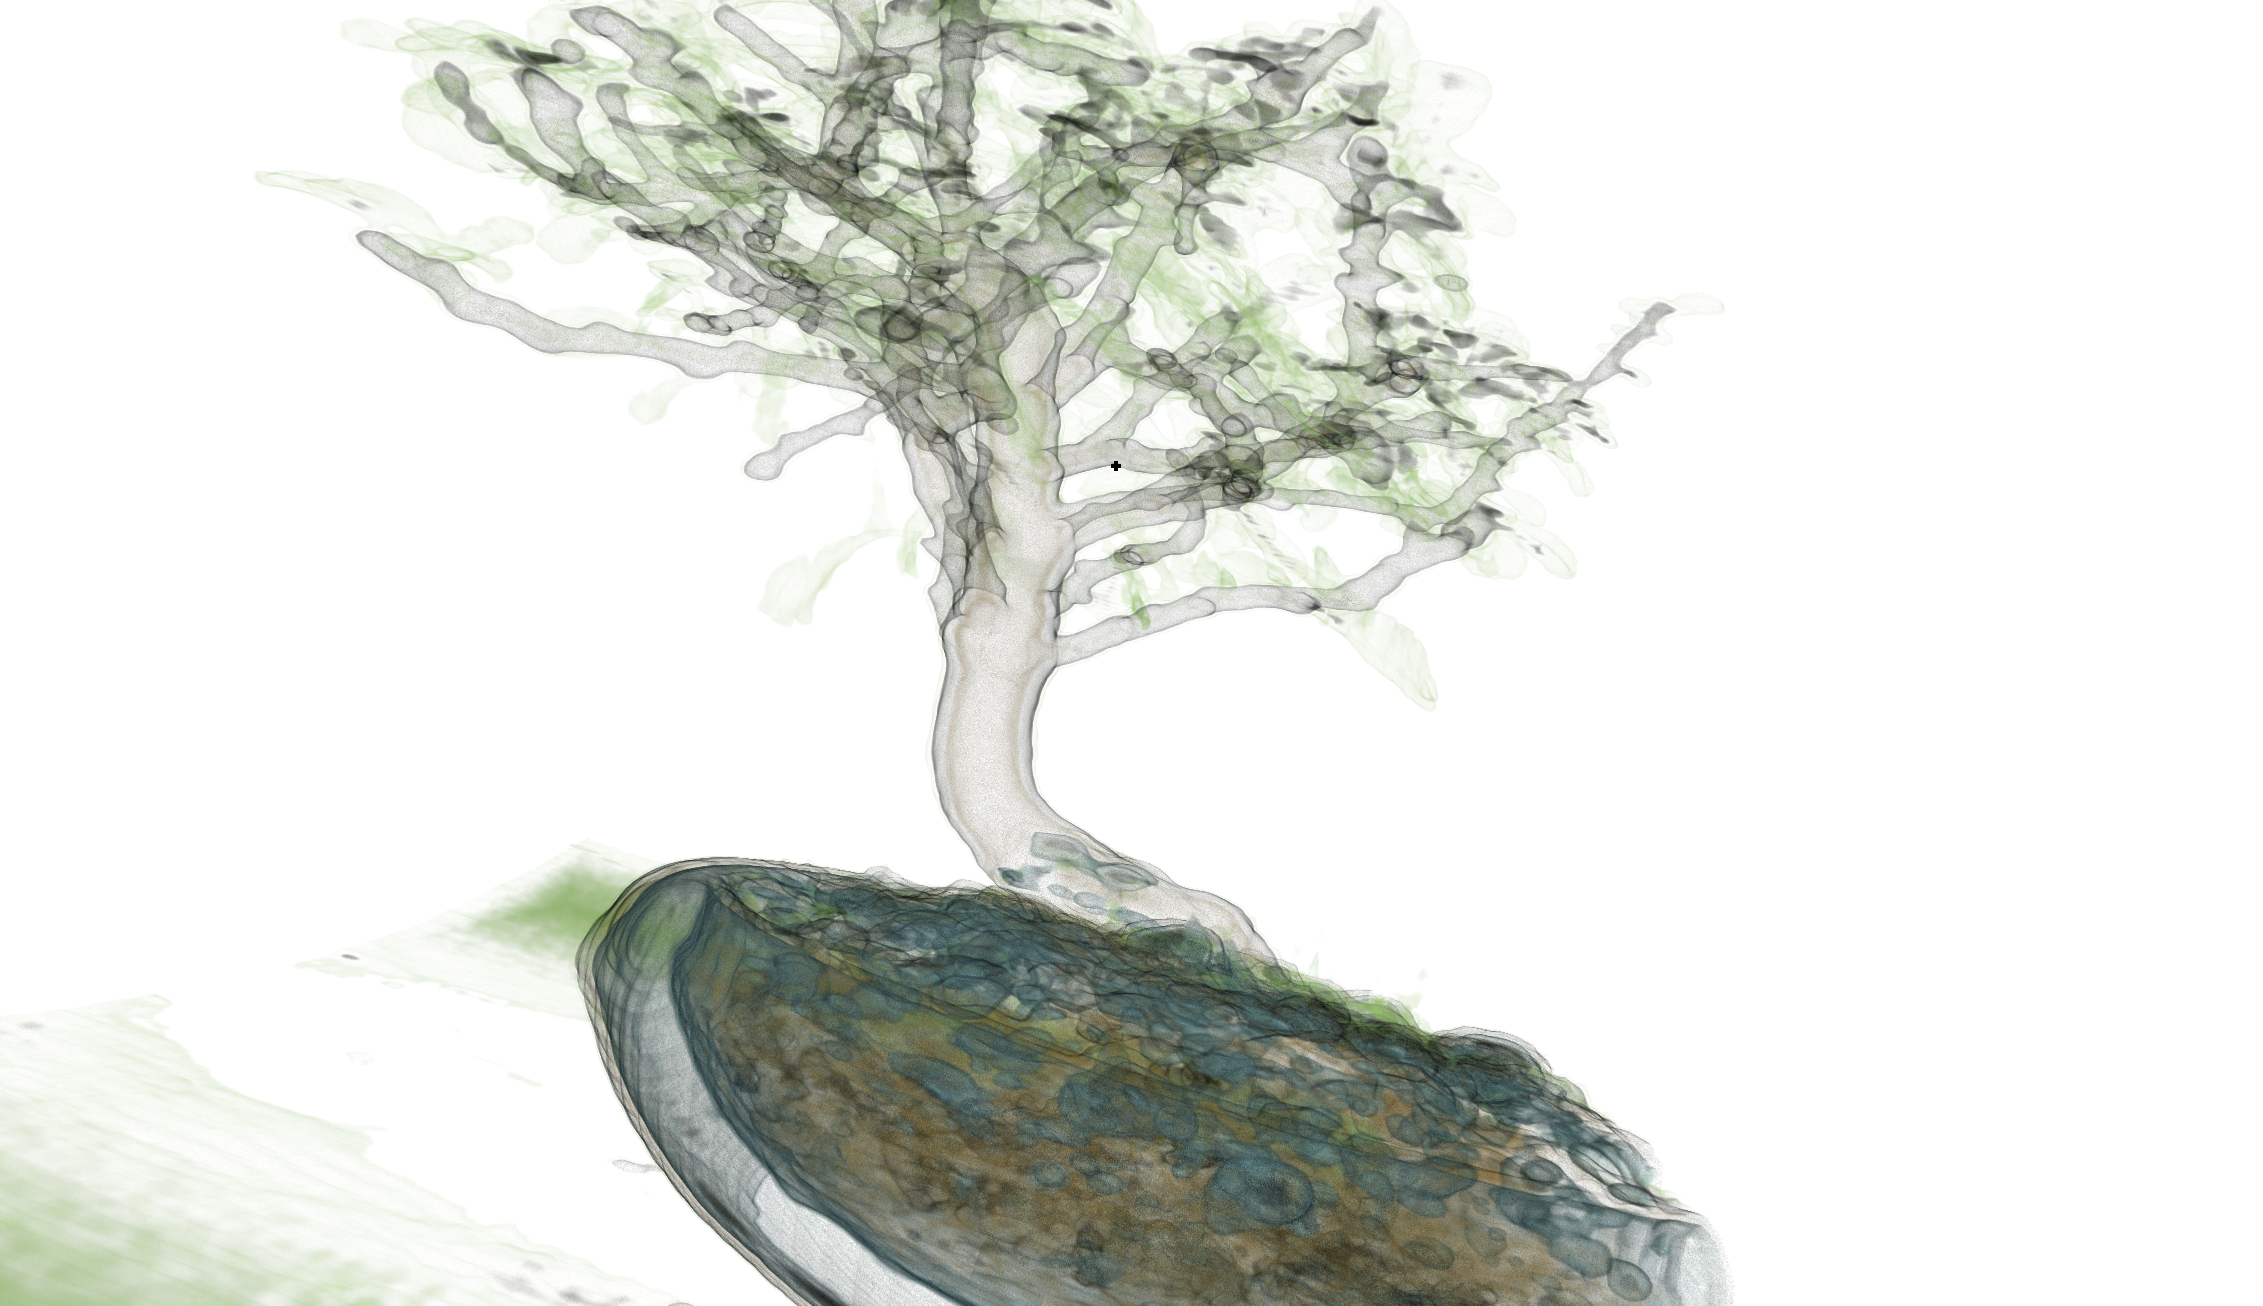
\includegraphics[width=\textheight]{../../Neue_Messungen/Bonsai/st_ors.png}
		\caption{Volumen Bonsai mit modifizierten Standard Raycast berechnet. Die Bildabtastrate beträgt $1$. Die Strahlabtastrate hat an der Mausposition einen Wert von $1,5$ und nimmt, abhängig von der Distanz zur Mausposition, bis zu einem Wert von $\frac{1,5}{4}$ ab.}
		\label{fig::res::bon_st_ors}
	\end{figure}
\end{landscape}

\subsubsection{MDC Raycast}\label{ss::res::mdc}
Der \emph{MDC} Raycast ist das Ergebnis des Arbeitspakets, aus dem Abschnitt \ref{ss::MDC}.
Die Abbildung \ref{fig::res::bon_mdc} zeigt das Volumen \emph{Bonsai}, welches mit dem \emph{MDC} Raycast erstellt wurde.
Das Bild wurde dabei aus der selben Perspektive und mit der gleichen Transferfunktion berechnet, wie dies auch in Abbildung \ref{fig::res::bon_st} der Fall war.

Die maximale Bildabtastrate in Abbildung \ref{fig::res::bon_mdc} hat einen Wert von $0,96$ statt einem Wert von $1,0$.
Damit wird einer leichten Verschiebung des Bildes, aufgrund der zwei unterschiedlichen Bildabtastraten, entgegengewirkt.
Die Anpassung der Bildabtastrate ist abhängig von der Auflösung des Bildes.

In diesem Fall, beim \emph{MDC} Raycast, wurden zwei Bilder berechnet, welche anschließend passend zusammengefügt wurden.
Das erste Bild wurde mit nur einem viertel der Auflösung berechnet, also der halben Bildabtastrate, und anschließend auf die ursprüngliche Auflösung interpoliert.
Das zweite Bild wurde mit der ursprünglichen Auflösung berechnet, dafür aber nur ein rechteckiger Ausschnitt an der Mausposition.
Anschließend wurde das zweite Bild an der Mausposition in das auf die normale Auflösung interpolierte erste Bild eingefügt.

An den Konturen der Abbildung \ref{fig::res::bon_mdc} ist ein leichter Abfall der Auflösung des Bildes zu erkennen.
Die Konturen, welche in Abbildung \ref{fig::res::bon_st} noch weich gezeichnet wurden, haben außerhalb des Rechtecks um die Mausposition nun Artefakte der Unterabtastung, wie zum Beispiel leichte Treppenstufen.
Innerhalb des Rechtecks sind die Konturen immer noch weich gezeichnet und es ist dort kein Unterschied zu Abbildung \ref{fig::res::bon_st} zu sehen.

Die Größe des Rechtecks beträgt $350$\,Pixel in x- und y-Richtung und ist groß genug, dass die Abnahme der Auflösung im äußeren Bereich, bei Fokussierung der Mausposition, nicht wahrnehmbar ist.
Wird bei aktivem Eyetracking anstelle der Mausposition die Blickposition verwendet, so ist der aktuell betrachtete Bereich immer hoch aufgelöst.
Ein Unterschied zwischen den beiden Bereichen fällt während einer Fokussierung kaum auf.
Wenn der Fokus langsam über das Bild wandert, kann man einen Unterschied zwischen den Auflösungen erkennen.
An dem Übergang des normal aufgelösten Bereichs zu dem Bereich mit der halben Auflösung kommt es während einer Bewegung an den Konturen des Volumen zu leichten Veränderungen.
Diese können die Aufmerksamkeit auf sich ziehen und daher auffallen.

Obwohl der Bereich außerhalb des Rechtecks mit nur einem Viertel der Auflösung innerhalb des Rechtecks berechnet wurde, ist die Bildqualität in diesem Bereich noch recht gut.
Da die Sehschärfe mit zunehmenden Winkel von der Fovea weg immer weiter abnimmt, könnte die Bildabtastrate außerhalb des Rechtecks vermutlich weiter gesenkt werden, ohne dass dies die Bildqualität bei der Verwendung eines Eye-Trackers beeinträchtigt.

Abbildung \ref{fig::res::bon_mdc_ors} zeigt die selbe Berechnung wie Abbildung \ref{fig::res::bon_mdc} aber mit einer variierten Strahlabtastrate.
Anders als in Abbildung \ref{fig::res::bon_st_ors}, in welcher ebenfalls die Strahlabtastrate auf die gleiche Weise über das Bild hinweg variiert wurde, macht sich in Abbildung \ref{fig::res::bon_mdc_ors} an zum Beispiel den Ästen, die geringere Strahlabtastrate bemerkbar.
Die Flächen der Äste erscheinen ein bisschen löchrig, da Voxel teilweise übersprungen werden.
Wird die Mausposition fokussiert, kann man dies, aufgrund der Distanz zum Blickpunkt, nicht wahrnehmen.

\begin{landscape}
	\begin{figure}
		\centering
		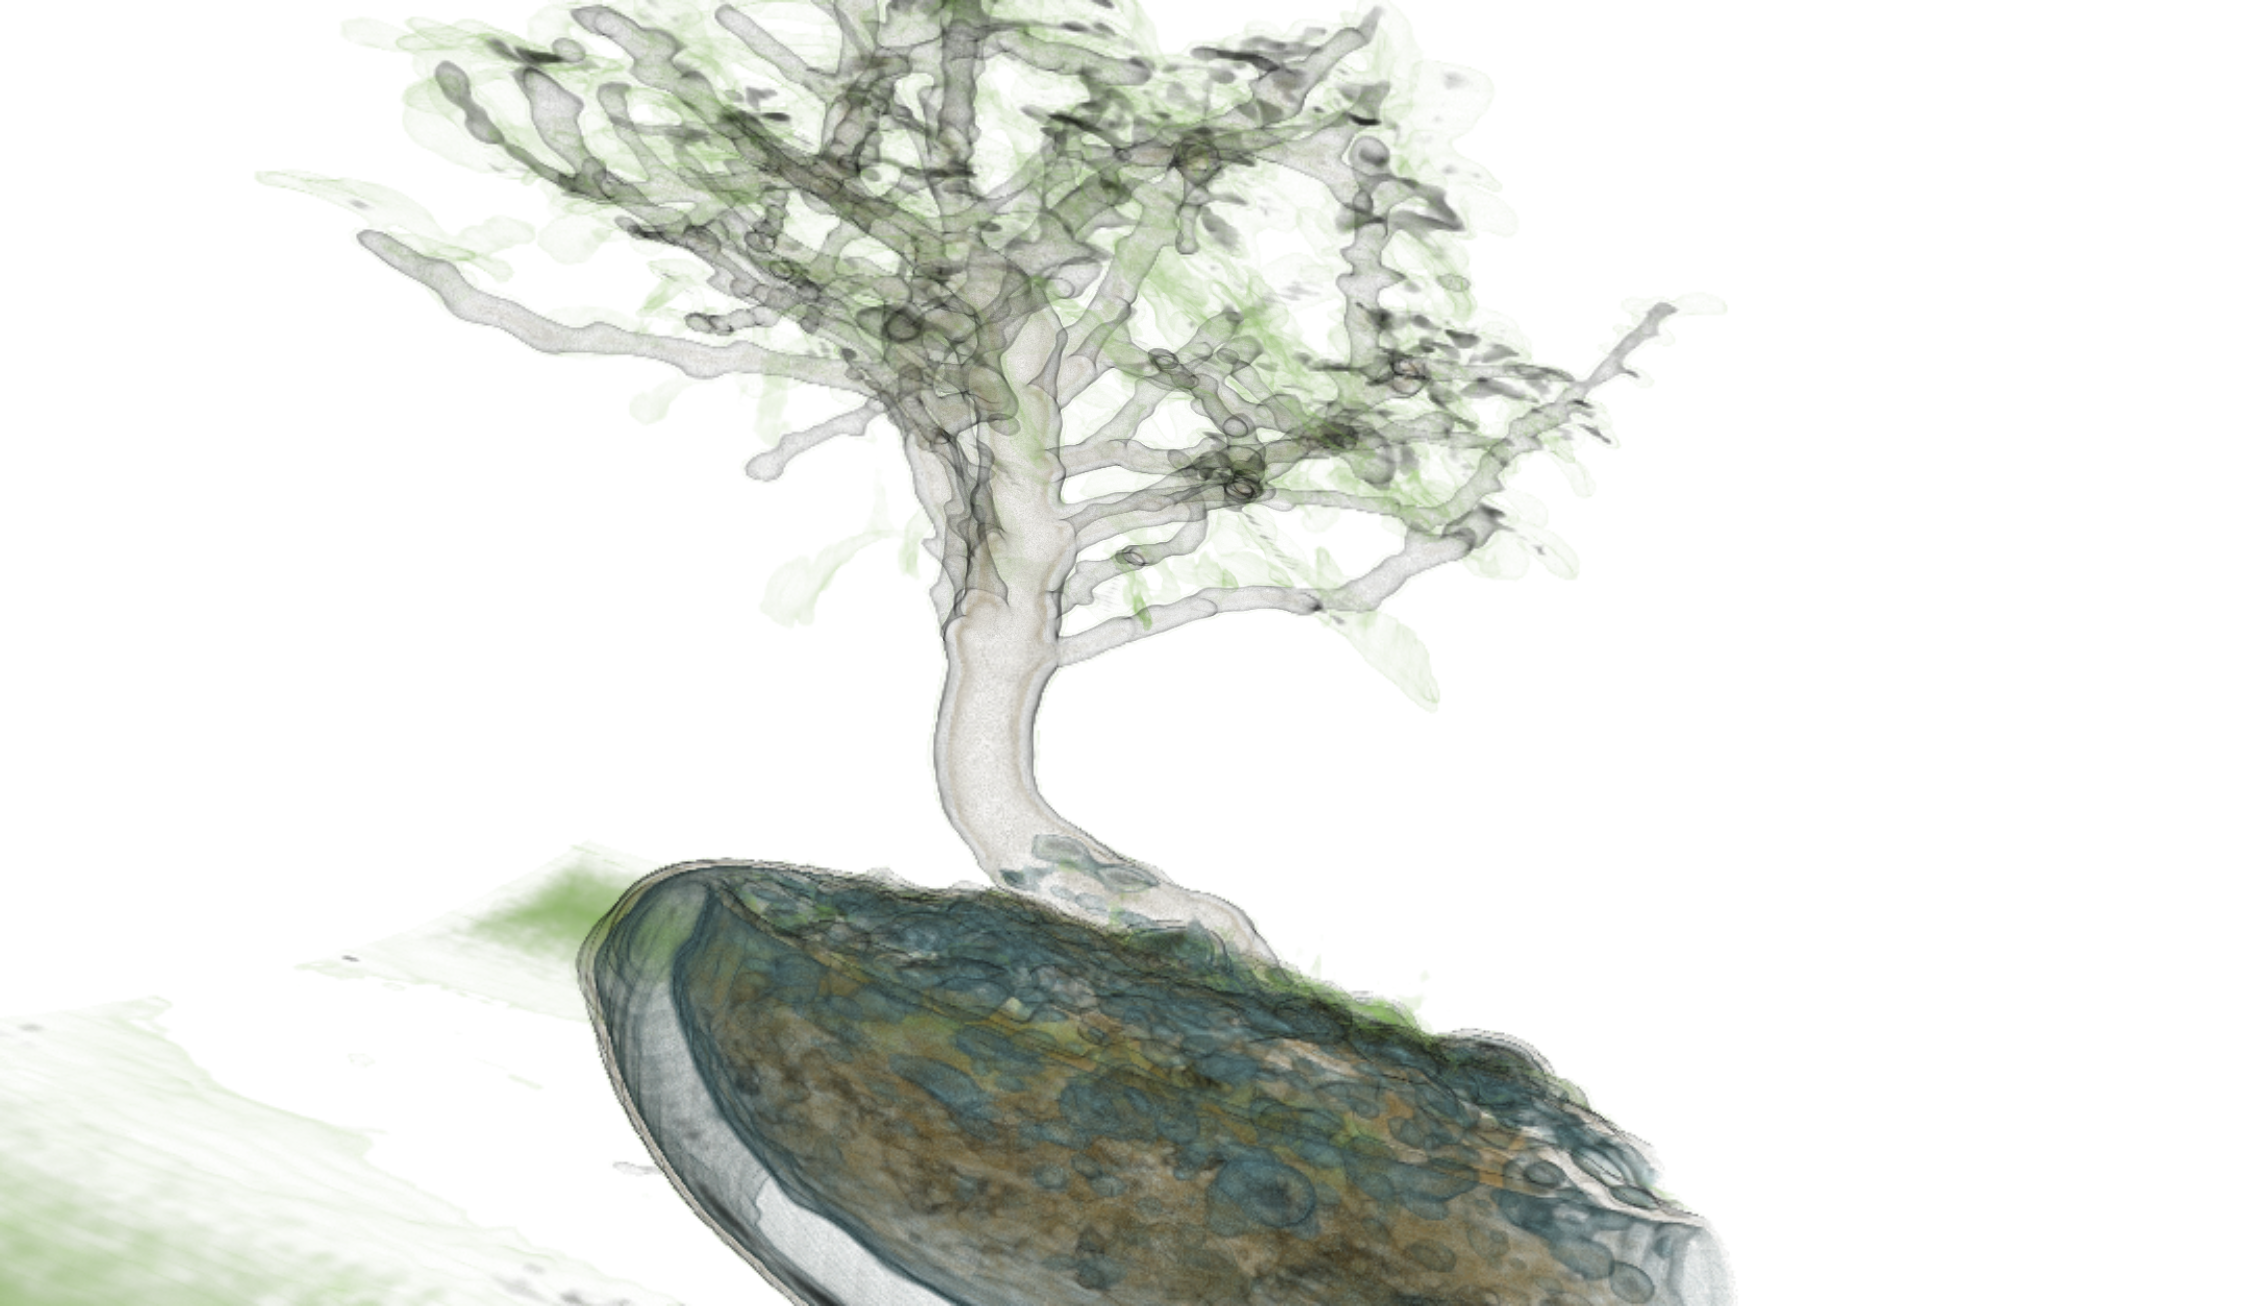
\includegraphics[width=1\textheight]{../../Neue_Messungen/Bonsai/mdc.png}
		\caption{Volumen Bonsai. Das Bild wurde mit dem \emph{MDC} Raycast berechnet. Ein kleiner Teil des Bildes, in Form eines Rechtecks, hat eine Bildabtastrate von $1,0$. Das restliche Bild hat nur eine Bildabtastrate von $0,5$. Die Strahlabtastrate beträgt für das ganze Bild $1.5$.}
		\label{fig::res::bon_mdc}
	\end{figure}
\end{landscape}

\begin{landscape}
	\begin{figure}
		\centering
		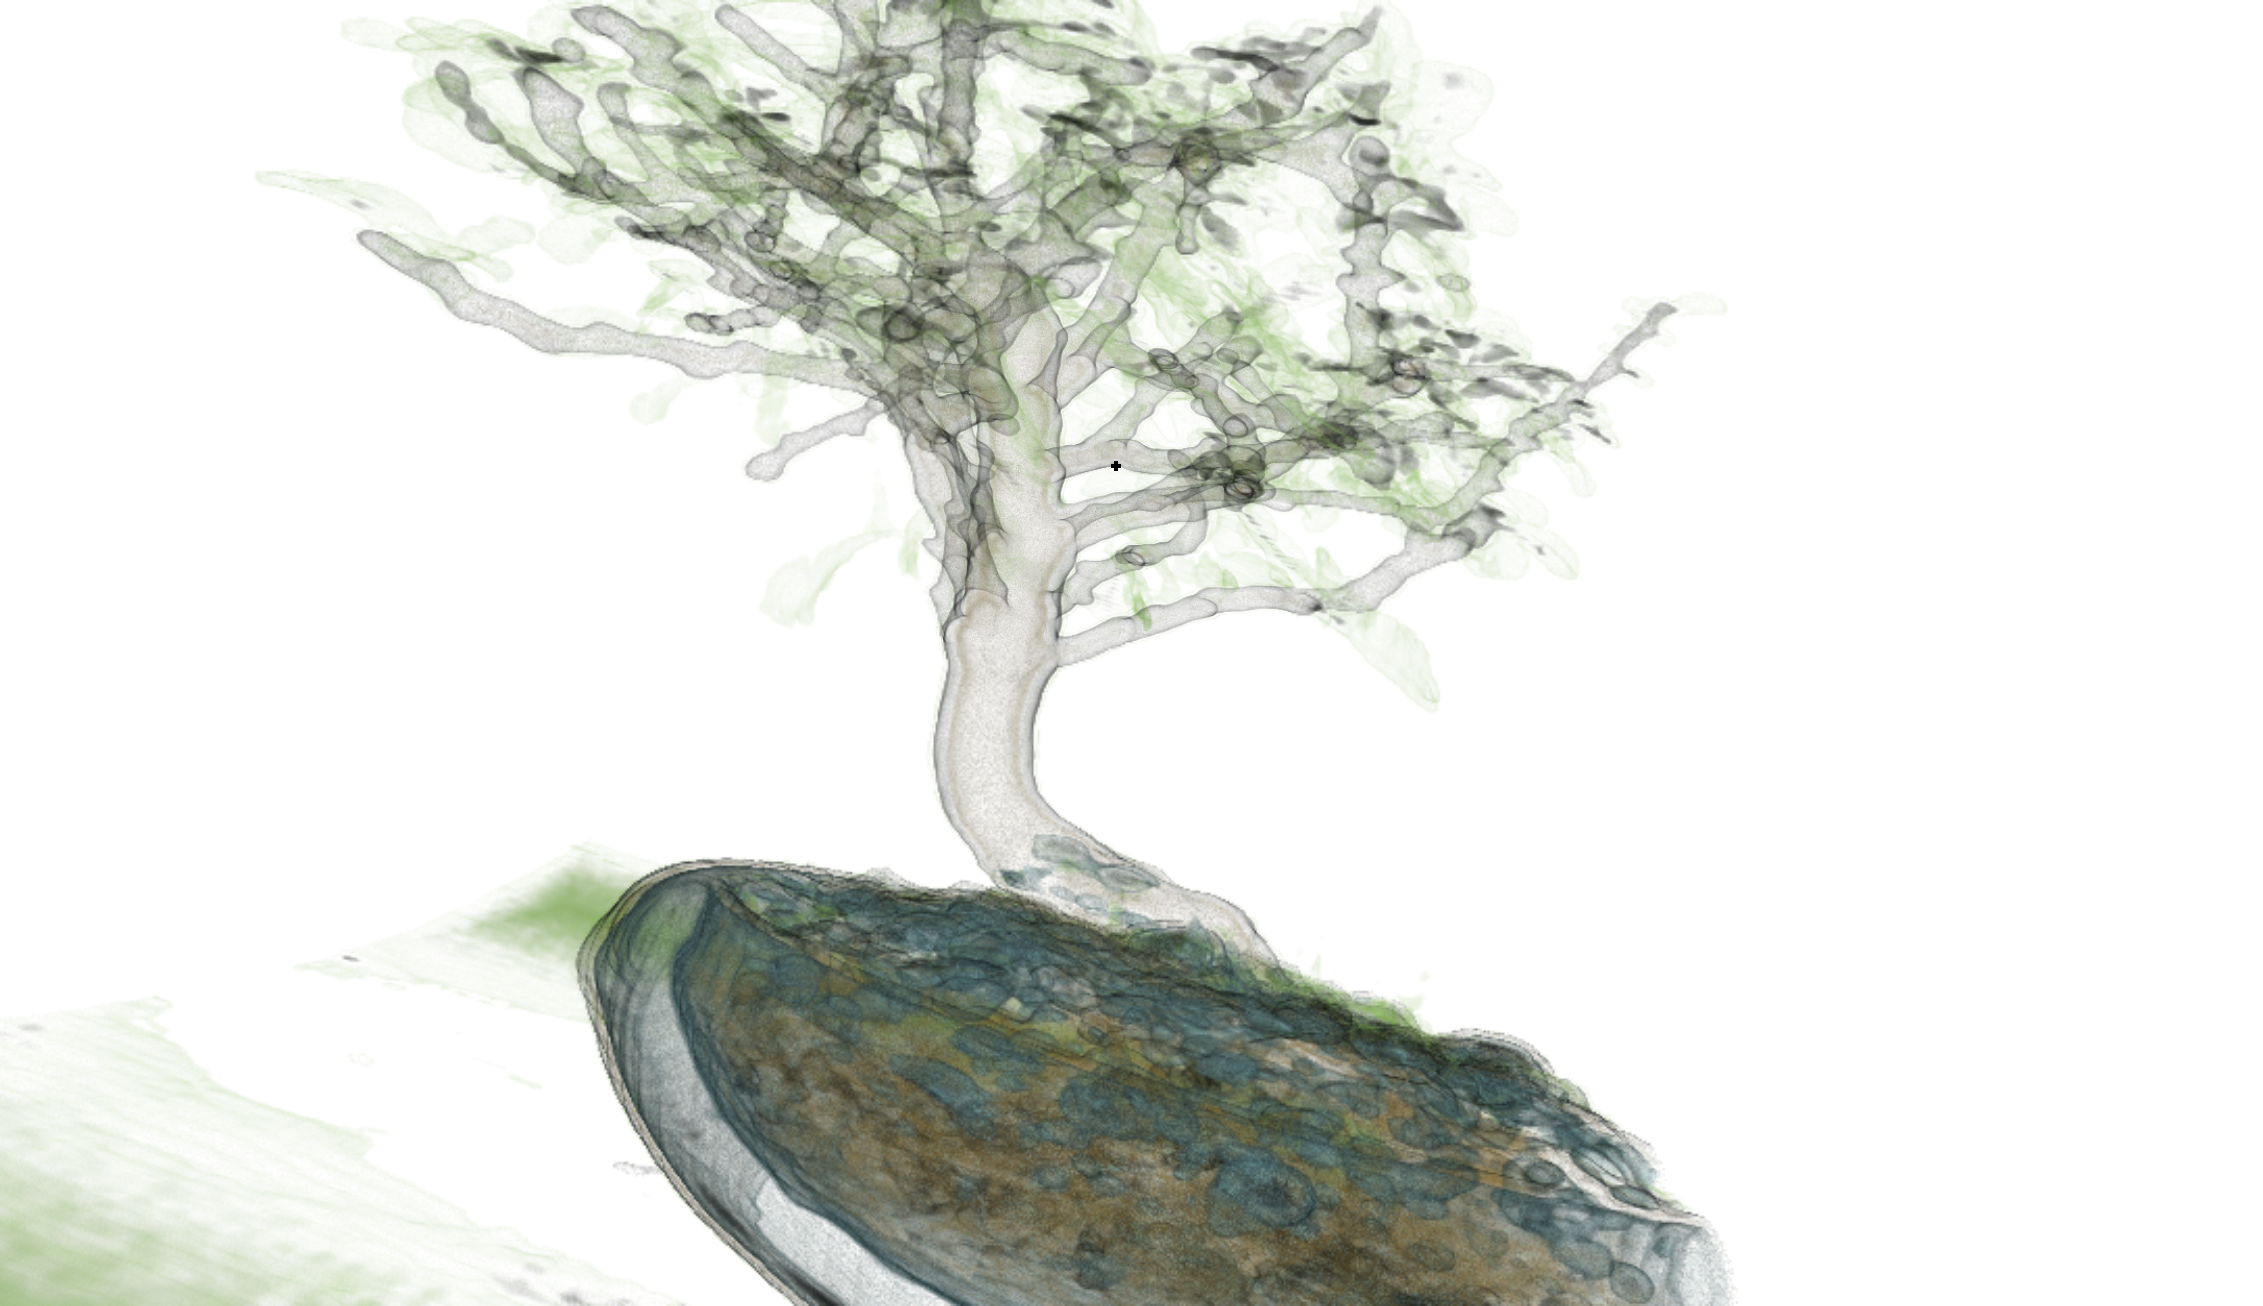
\includegraphics[width=1\textheight]{../../Neue_Messungen/Bonsai/mdc_ors.png}
		\caption{Volumen Bonsai. Das Bild wurde mit dem \emph{MDC} Raycast berechnet. Ein kleiner Teil des Bildes, in Form eines Rechtecks, hat eine Bildabtastrate von $1,0$. Das restliche Bild hat nur eine Bildabtastrate von $0,5$. Die Strahlabtastrate hat an der Mausposition einen Wert von $1,5$ und nimmt, abhängig von der Distanz zur Mausposition, bis zu einem Wert von $\frac{1,5}{4}$ ab.}
		\label{fig::res::bon_mdc_ors}
	\end{figure}
\end{landscape}

\subsubsection{DDC Raycast}\label{ss::res::ddc}
Der \emph{DDC} Raycast ist das Ergebnis des Arbeitspakets aus dem Abschnitt \ref{ss::DDC}.
Abbildung \ref{fig::res::bon_ddc} zeigt das Volumen \emph{Bonsai}, welches mit dem \emph{DDC} Raycast erstellt wurde.
Das Bild wurde aus der selben Perspektive und mit der gleichen Transferfunktion berechnet, wie in den Abbildungen \ref{fig::res::bon_st} und \ref{fig::res::bon_mdc}.
Die maximale Bildabtastrate ist $1$.
Diese nimmt in zwei Stufen nach außen hin ab.

Beim \emph{DDC} Raycast wurde nur ein Aufruf des Raycasts gestartet und die Work-Items und ihre entsprechenden Strahlen auf verschiedene Bildpunkte abgebildet.
Das gesamte Bild wurde in einem zweiten Kernel Aufruf interpoliert.
Innerhalb eines kleinen Bereichs in der Form einer Ellipse um den Blickpunkt herum hat das Bild eine Bildabtastrate von $1$, dass heißt jeder Pixel entspricht einem Farbwert der Auswertung eines Strahls.
Außerhalb von diesem Bereich aber innerhalb einer zweiten größeren und umschließenden Ellipse hat das Bild in x- und y-Richtung eine Bildabtastrate von $\frac{1}{2}$.
Das heißt, dass in x- und y-Richtung nur für jedes zweiten Pixel ein Strahl ausgewertet wird.
In dem äußersten Bereich beträgt die Bildabtastrate in x- und y-Richtung $\frac{1}{7}$.
Es wird also in jedem $7\times7$\,Pixel-Feld nur ein Strahl ausgewertet.
Die die Farbwerte der Pixel, die selbst nicht durch einen Strahl bestimmt wurden, wurden durch vier umliegende Farbwerte von Strahlen bilinear interpoliert.

In Abbildung \ref{fig::res::bon_ddc} ist deutlich zu sehen, dass der Großteil des Bildes eine geringe Auflösung hat.
In dem am niedrigsten abgetasteten Bereich sind an den Konturen, insbesondere die der Äste, deutliche Merkmale der Unterabtastung zu sehen.
In Abbildung \ref{fig::res::bon_st} und \ref{fig::res::bon_mdc} verlaufen die Konturen der Äste noch diagonal und sind relativ weich gezeichnet, hier haben sie starke Treppeneffekte.
Manche Konturen sind auch teilweise unterbrochen.

In dem mittleren Bereich ist die Bildqualität recht gut und das Bild scharf zu erkennen.
Trotzdem hat das Bild hier nur ein Viertel der Auflösung.
Den Übergang zwischen dem mittleren und inneren Bereich, welcher die normale Auflösung hat, ist kaum zu erkennen.
Aufgrund des starken Abfalls der Bildabtastrate vom mittleren zum äußeren Bereich, fällt dieser Übergang stärker auf.

Bei aktivem Eyetracking wird anstelle der Mausposition die aktuelle Blickposition verwendet.
Der Fokus liegt bei aktivem Eyetracking nun im Zentrum des inneren Bereichs, dieser wurde hier mit der Mausposition simuliert und ist als schwarzes Kreuz eingezeichnet.
Der innere Bereich ist groß genug, so dass der Abfall der Bildabtastrate zum mittleren Bereich nicht auffällt.
Zusammen ergeben der innere und mittlere Bereich den Teil des Bildes, in welchem das Bild scharf zu sehen ist.
Dieser ist ausreichend groß, dass der Bereich an und um dem Blickpunkt immer scharf wahrgenommen wird.
Anders als in Abbildung \ref{fig::res::bon_mdc}, ist es in Abbildung \ref{fig::res::bon_ddc} auch wenn der innere und mittlere Bereich auf den Blickpunkt zentriert sind, auffallend, dass der äußere Bereich mit einer deutlich niedrigeren Bildabtastrate berechnet wurde.
Die grundlegenden Konturen des Bildes können aber im äußeren Bereich noch erkannt werden wodurch das Identifizieren von interessanten Objekten immer noch möglich ist.

Abbildung \ref{fig::res::bon_ddc_ors} zeigt die selbe Berechnung wie Abbildung \ref{fig::res::bon_ddc} aber mit einer variierten Strahlabtastrate, wie sie in Abbildung \ref{fig::res::bon_st_ors} und \ref{fig::res::bon_mdc_ors} auch der Fall war.
Wie in Abbildung \ref{fig::res::bon_mdc_ors} erscheinen Teile, der von der Mausposition weiter entfernten Objekte, löchrig.
Der Unterschied zwischen variierter und nicht-variierter Strahlabtastrate fällt bei der DDC Raycast Methode ein wenig stärker auf, als bei der MDC Raycast Methode.
Trotzdem ist beeinflusst die viel niedrigere Auflösung im äußeren Bereich die Bildqualität viel maßgebender, als die reduziert Strahlabtastrate, so dass diese kaum mehr die Wahrnehmung beeinträchtigt.
Dies ist noch weniger der Fall, wenn die Mausposition fokussiert wird.

\begin{landscape}
	\begin{figure}
		\centering
		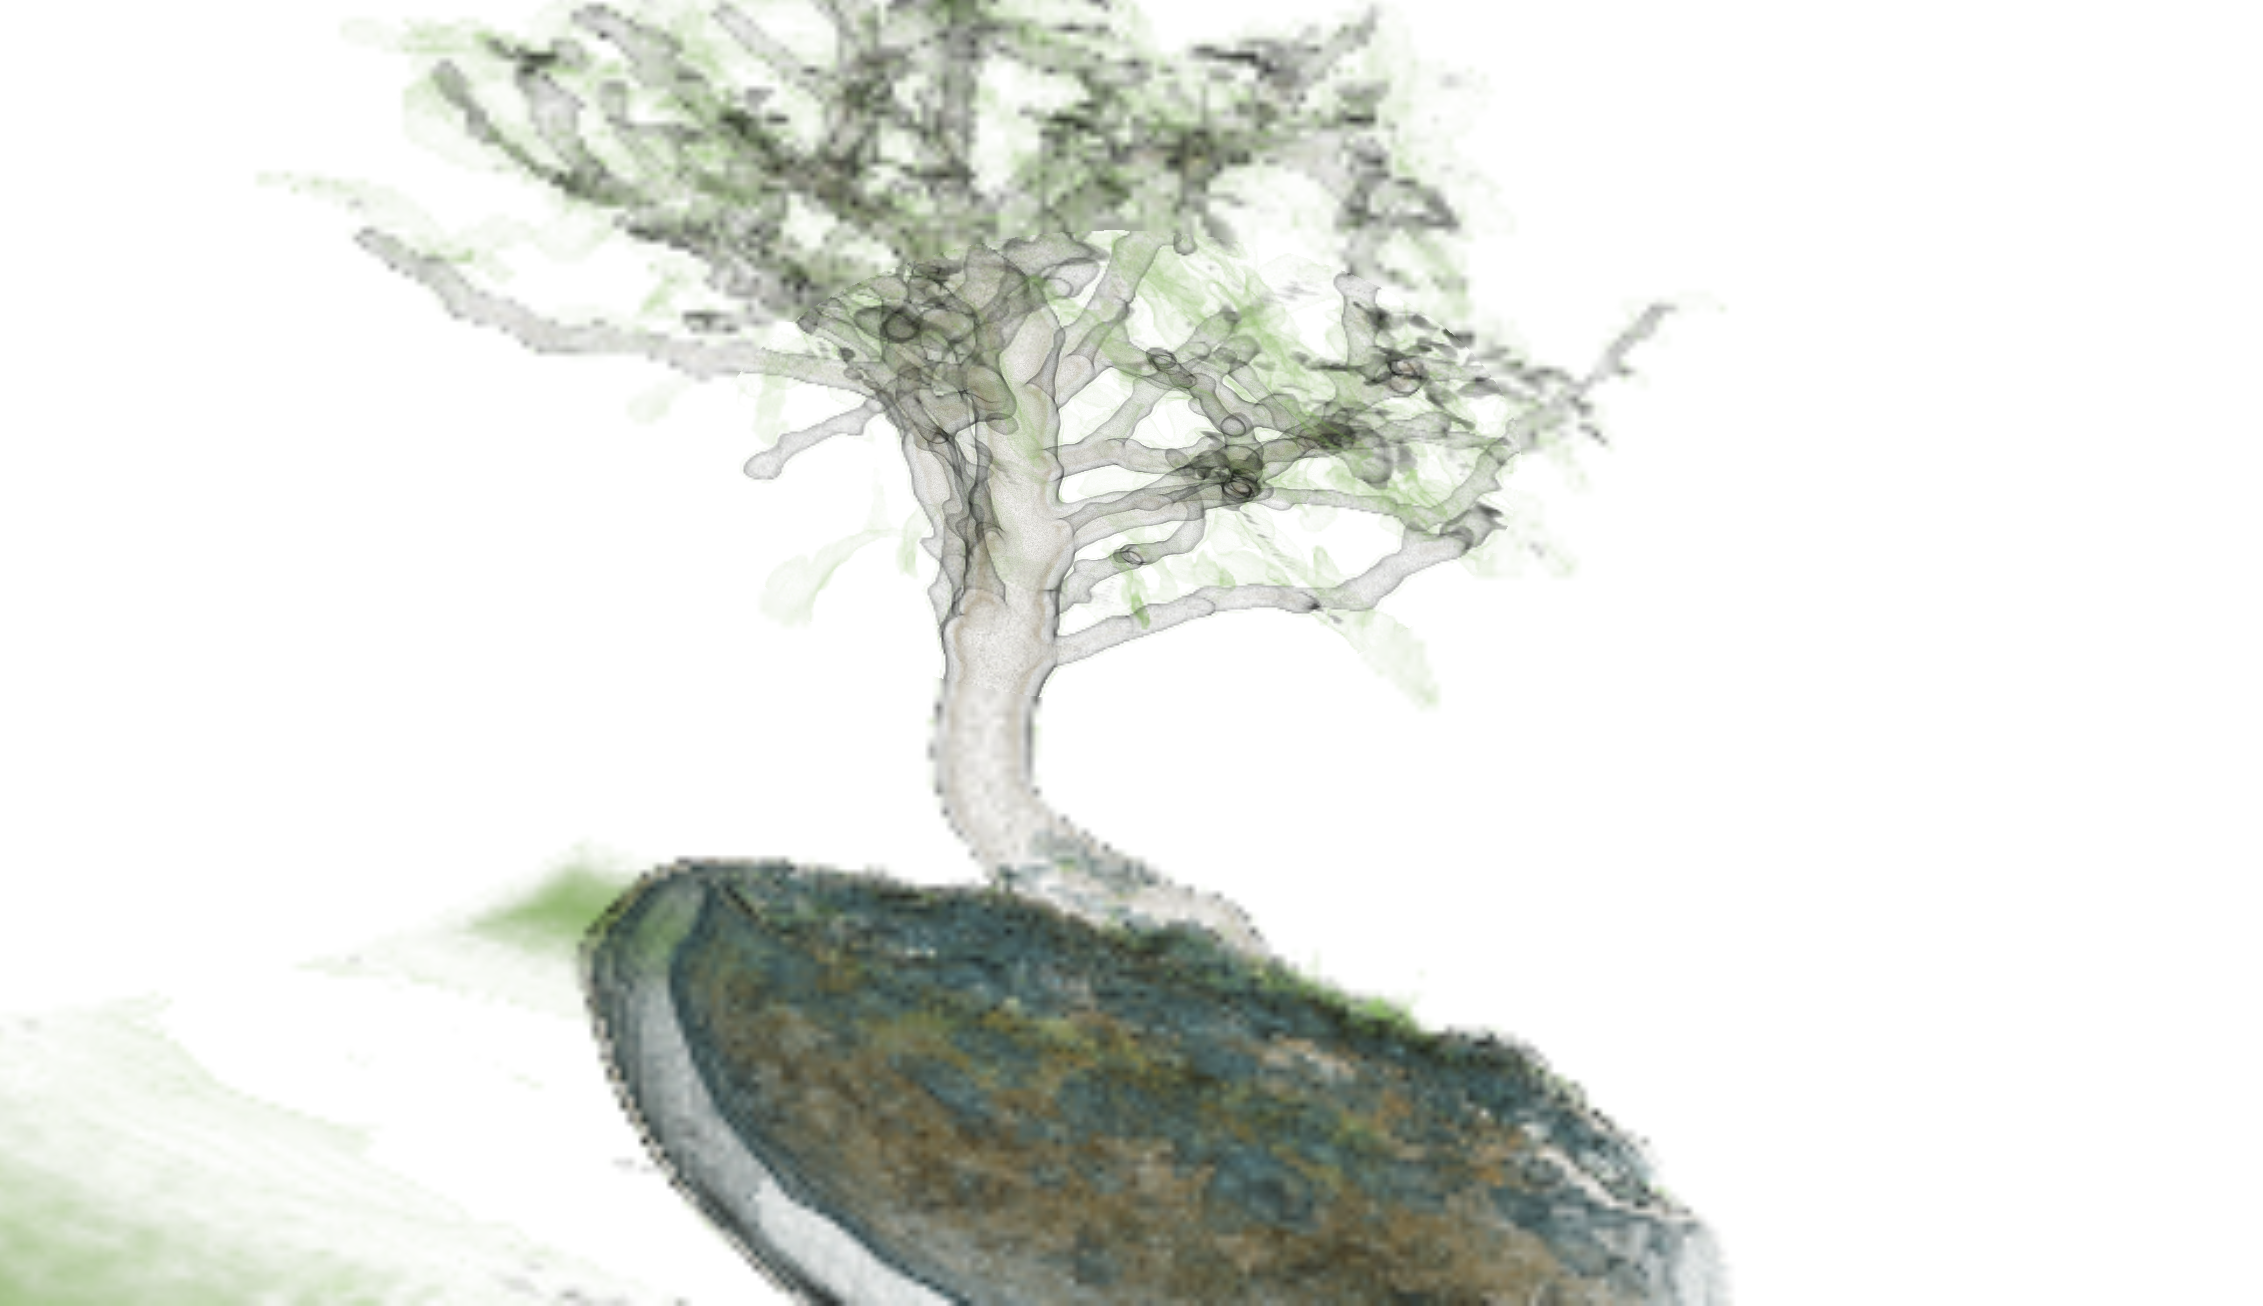
\includegraphics[width=1\textheight]{../../Neue_Messungen/Bonsai/ddc.png}
		\caption{Volumen Bonsai mit \emph{DDC} Raycast berechnet. Die Bildabtastrate nimmt nach außen hin in zwei Schritten ab. An der Mausposition hat sie den höchsten Wert von $1,0$. Etwas weiter außen einen Wert von $0,5$ und noch weiter außen hat sie den niedrigsten Wert von $\frac{1}{7}$. Die Strahlabtastrate beträgt für das ganze Bild $1.5$.}
		\label{fig::res::bon_ddc}
	\end{figure}
\end{landscape}

\begin{landscape}
	\begin{figure}
		\centering
		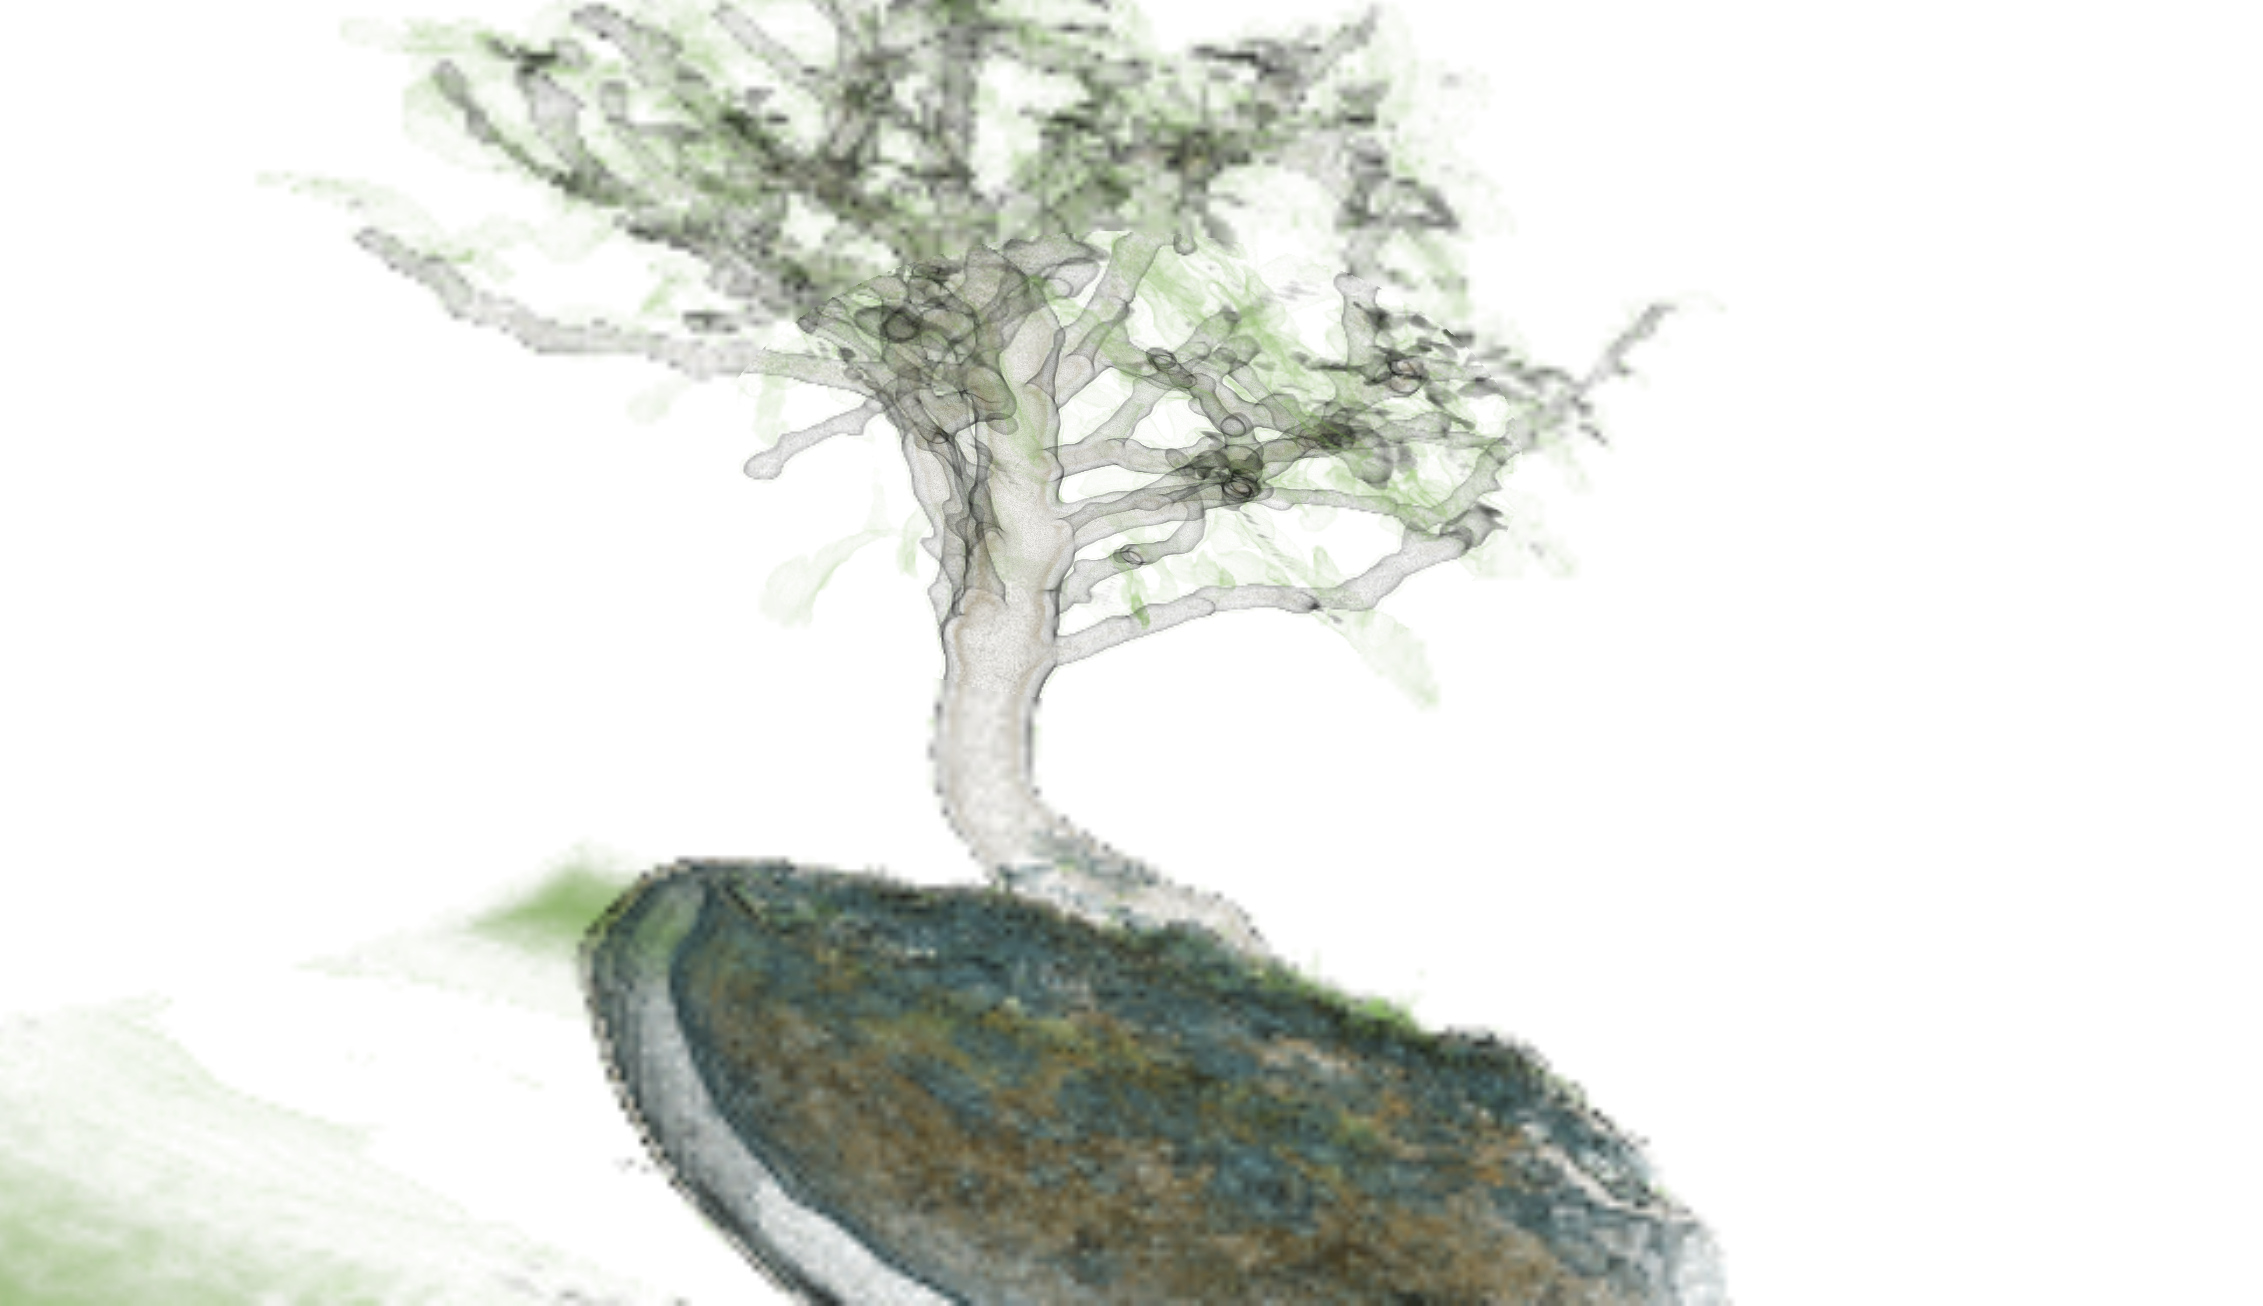
\includegraphics[width=1\textheight]{../../Neue_Messungen/Bonsai/ddc_ors.png}
		\caption{Volumen Bonsai mit \emph{DDC} Raycast berechnet. Die Bildabtastrate nimmt nach außen hin in zwei Schritten ab. An der Mausposition hat sie den höchsten Wert von $1,0$, weiter außen einen Wert von $0,5$, dann einen Wert von $\frac{1}{7}$. Die Strahlabtastrate hat an der Mausposition einen Wert von $1,5$ und nimmt, abhängig von der Distanz zur Mausposition, bis zu einem Wert von $\frac{1,5}{4}$ ab.}
		\label{fig::res::bon_ddc_ors}
	\end{figure}
\end{landscape}

\subsubsection*{Direkter Vergleich}
Abbildung \ref{fig::res::sn_comp_st_123} zeigt eine Berechnung des zweiten Volumens, welche mit dem Standard Raycast und ohne einer variierten Strahlabtastrate berechnet wurde.
Anders als das erste Volumen, welches ein ct-scan ist, ist dieses der $1353$-te Zeitschritt aus der Simulation einer \emph{shock wave formation in core-collapse supernova} von John Blondin, NCSU.
Es hat eine Auflösung von $432\times432\times432$\,Voxel, welche ebenfalls in x-, y- und z-Richtung eine Skalierung von $1,0$ haben.
Die Dichte der Voxel gibt die physikalische Entropie an der Position in der Simulation an.

In Abbildung \ref{fig::res::sn_comp_st_123} sind drei Kästchen eingezeichnet und nummeriert.
Für jede der Berechnungsmethoden wurde das Volumen mit der gleichen Transferfunktion und Perspektive beziehungsweise Kameraausrichtung berechnet.
Für jede der Berechnungen sind die drei Ausschnitte vergrößert worden und nebeneinander der Reihe nach aufgeführt.
Die Mausposition für die jeweiligen Berechnungen war dabei immer an der selben Position und ist jeweils in Ausschnitt $2$ eingezeichnet.

Ausschnitt $1$ liegt etwas weiter weg von der Mausposition aber circa am Übergang des mittleren Bereichs zum äußeren Bereich des \emph{DDC} Raycasts.
Die Strahlabtastrate wäre entsprechend in Ausschnitt $1$ ein wenig geringer, als an der Mausposition, falls eine Methode mit variierte Strahlabtastrate verwendet wurde.
Ausschnitt $2$ enthält die Mausposition und ist dementsprechend jeweils im inneren Bereich mit einer Bildabtastrate von $1$.
Die Strahlabtastrate ist hier ebenfalls fast maximal bei $1,5$.
Ausschnitt $3$ liegt relativ zur Auflösung des Bildes weit von der Mausposition entfernt.
Die Bildabtastrate beträgt hier für den Standard Raycast $1$, für den \emph{MDC} Raycast $\frac{1}{2}$ und für den \emph{DDC} Raycast $\frac{1}{7}$.
Wird eine Methode mit variierte Strahlabtastrate verwendet, so hat diese in Ausschnitt $3$ fast den minimalen Wert von $\frac{1,5}{4}$.

Da die Mausposition sich innerhalb des zweiten Ausschnitts befindet, ist die Strahlabtastrate und die Bildabtastrate hier immer fast maximal, so dass Ausschnitt $2$ in den verschiedenen Methoden fast identisch ist.
Auch ist hier auffallend, dass obwohl, dass die Strahlabtastrate in Ausschnitt $3$ bei der Verwendung des selben Raycast mit einmal konstanter Strahlabtastrate und variierter Strahlabtastrate, sehr unterschiedlich ist, dies sich bei diesem Bild aber kaum auswirkt und nicht wahrgenommen wird.
Womöglich liegt das daran, dass durch die Transferfunktion in diesem Volumen eher größere und dickere Strukturen hervorgehoben wurden und daher selbst bei einer deutlich geringeren Strahlabtastrate diese Strukturen genügend oft abgetastet wurden.

Die eigentlichen Unterschiede sieht man bei der Verwendung verschiedener Raycasts besonders in Ausschnitt $1$.
So ist mit dem Standard Raycast der gesamte Ausschnitt $1$ scharf zu sehen (siehe Abbildung \ref{fig::res::sn_comp_st_ors}), während bei dem \emph{MDC} Raycast an den Konturen am Rand des Volumens zu sehen ist, dass diese leicht unschärfer sind (siehe Abbildung \ref{fig::res::sn_comp_mdc_ors}).
Ausschnitt $3$ unterscheidet sich hier zwischen dem Standard Raycast und dem \emph{MDC} Raycast kaum.

Ein wesentlicher Unterschied ist sowohl in Ausschnitt $1$ als auch in Ausschnitt $3$ zwischen dem \emph{DDC} Raycast und dem \emph{MDC} sowie dem Standard Raycast wahrnehmbar.
Man kann sehen, dass der äußere Bereich des \emph{DDC} Raycast (siehe Abbildung \ref{fig::res::sn_comp_ddc_ors}), deutlich unschärfer ist, als der äußere Bereich des \emph{MDC} Raycast (siehe Abbildung \ref{fig::res::sn_comp_mdc_ors}).

\begin{figure}
	\centering
	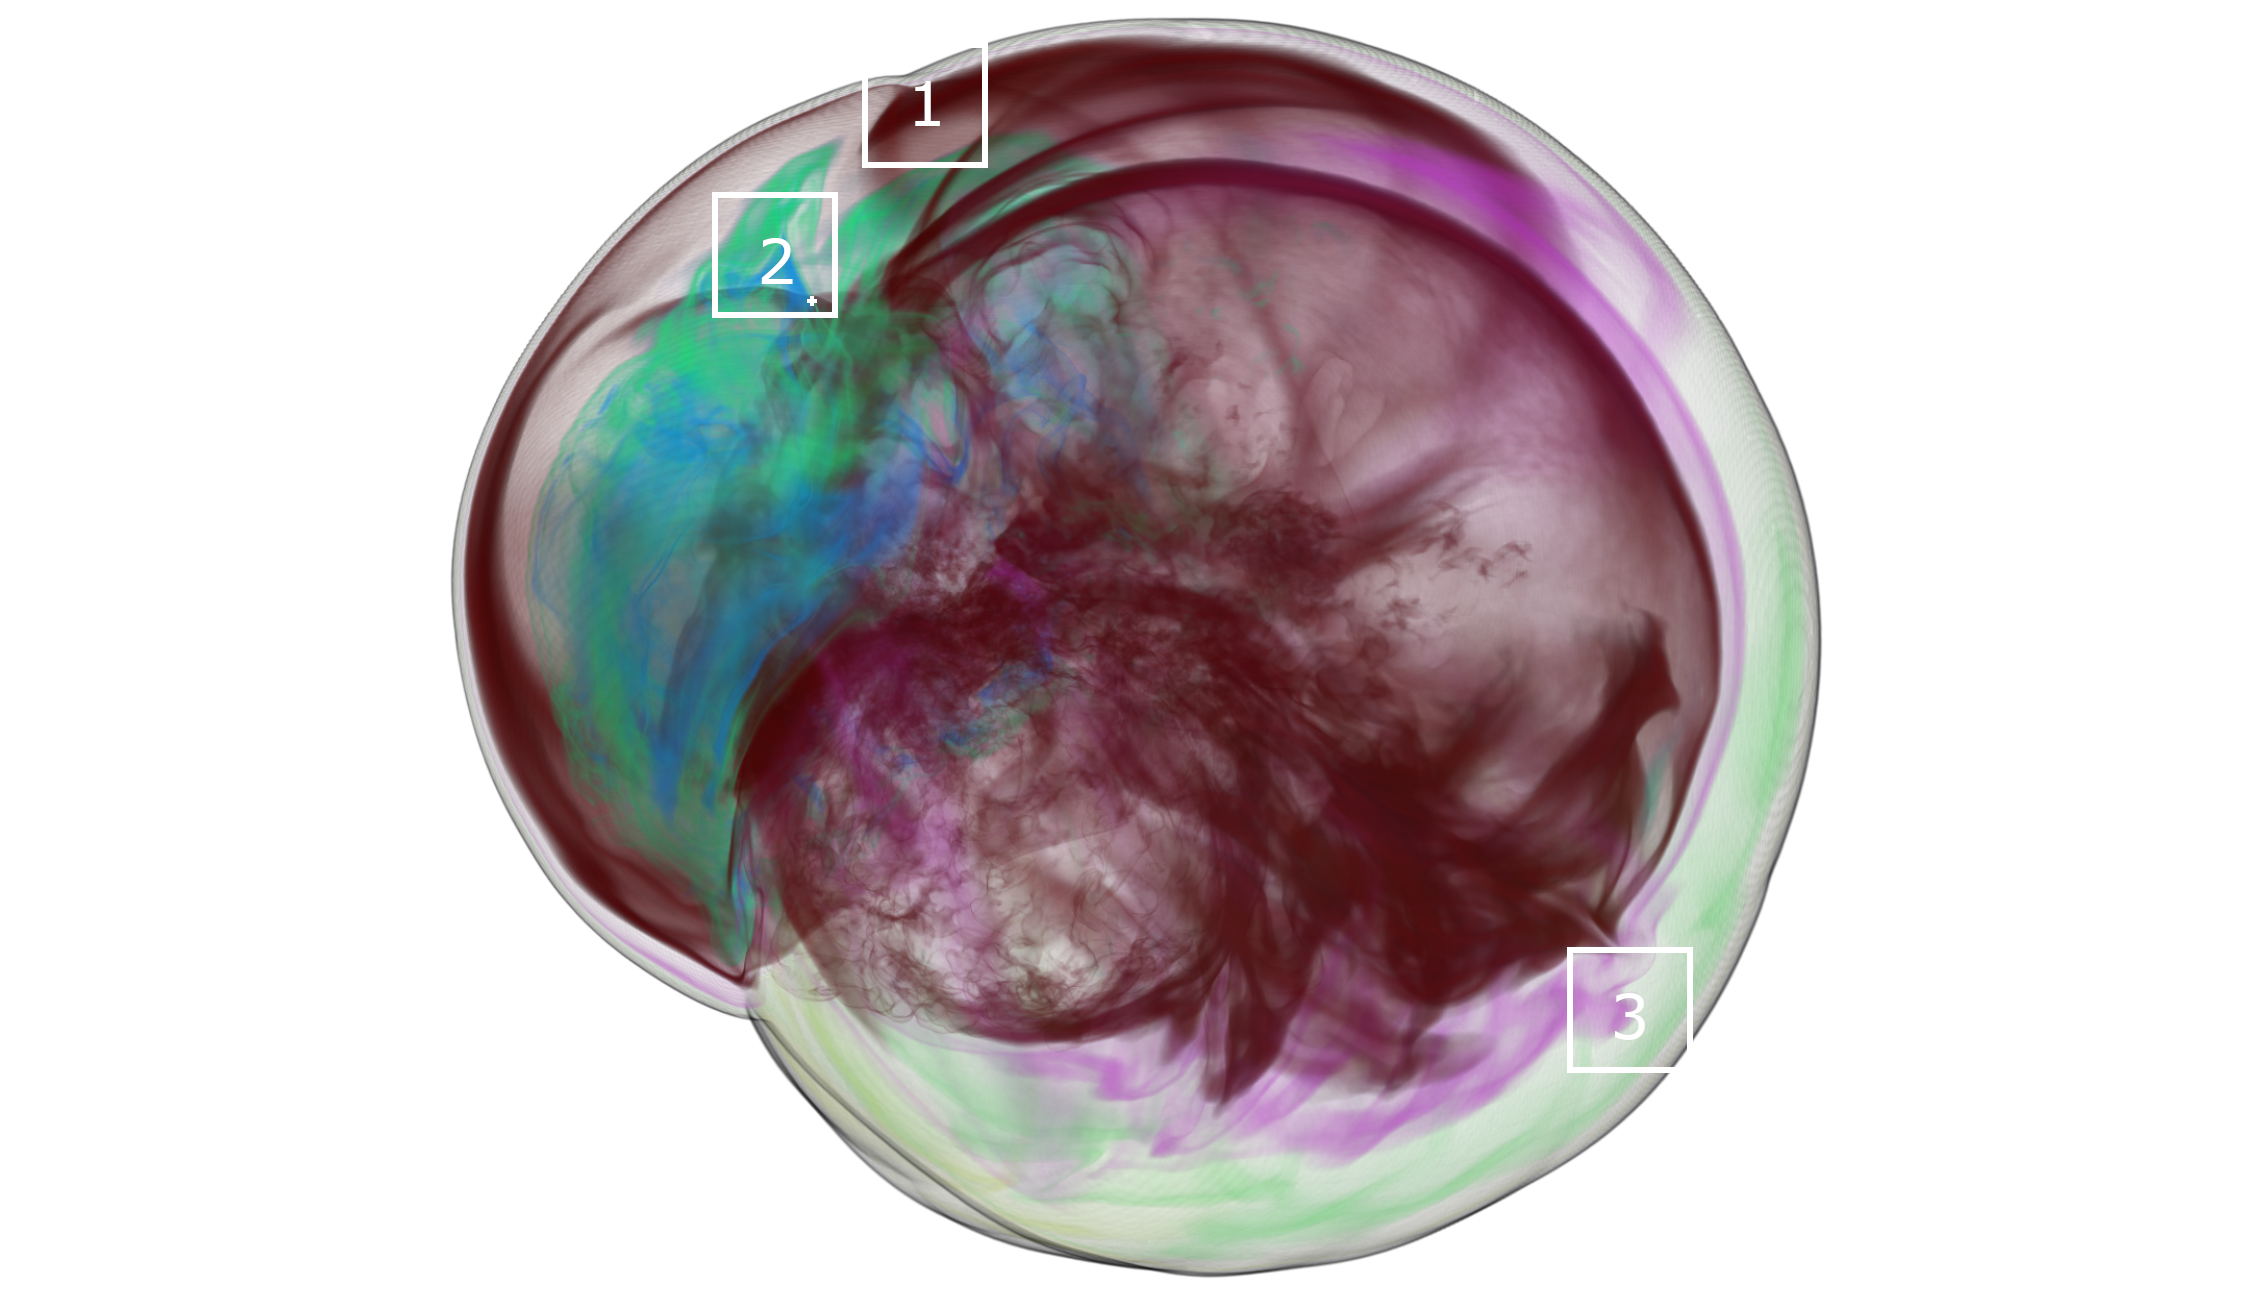
\includegraphics[width=0.7\textwidth]{../../Neue_Messungen/Supernova/cut/st/st_123.png}
	\caption{Ein Zeitschritt der Supernova mit dem Standard Raycast berechnet. Die Bildabtastrate beträgt für das ganze Bild $1$. Die Strahlabtastrate beträgt für das ganze Bild $1,5$. die Mausposition und drei nummerierte Quadrate sind eingezeichnet, die Positionen der Quadrate werden im folgenden Vergleich verwendet.}
	\label{fig::res::sn_comp_st_123}
\end{figure}

\begin{figure}[]
	\centering
	\begin{minipage}[t]{0.3\textwidth}
		\centering
		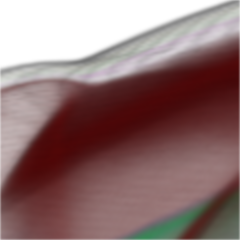
\includegraphics[width=1\textwidth]{../../Neue_Messungen/Supernova/cut/st/st_1.png}
		% \caption*{Quadrat 1 vergrößert dargestellt.}
		% \label{fig::res::sn_comp_st_1}
	\end{minipage}
	\hfill
	\begin{minipage}[t]{0.3\textwidth}
		\centering
		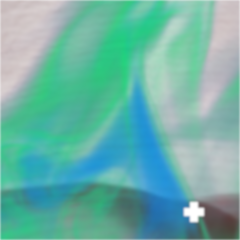
\includegraphics[width=1\textwidth]{../../Neue_Messungen/Supernova/cut/st/st_2.png}
		% \caption*{Quadrat 2 vergrößert dargestellt.}
		% \label{fig::res::sn_comp_st_2}
	\end{minipage}
	\hfill
	\begin{minipage}[t]{0.3\textwidth}
		\centering
		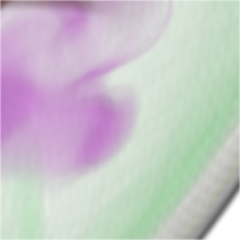
\includegraphics[width=1\textwidth]{../../Neue_Messungen/Supernova/cut/st/st_3.png}
		% \caption*{Quadrat 3 vergrößert dargestellt.}
		% \label{fig::res::sn_comp_st_3}
	\end{minipage}
	\caption{Supernova mit Standard Raycast und ohne variierter Strahlabtastrate berechnet.}
	\label{fig::res::sn_comp_st}
\end{figure}

\begin{figure}[]
	\centering
	\begin{minipage}[t]{0.3\textwidth}
		\centering
		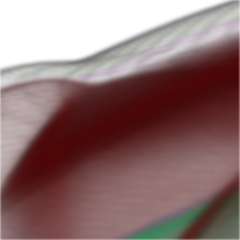
\includegraphics[width=1\textwidth]{../../Neue_Messungen/Supernova/cut/st_ors/st_ors_1.png}
		% \caption*{Quadrat 1 vergrößert dargestellt.}
		% \label{fig::res::sn_comp_st_ors_1}
	\end{minipage}
	\hfill
	\begin{minipage}[t]{0.3\textwidth}
		\centering
		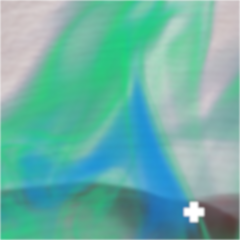
\includegraphics[width=1\textwidth]{../../Neue_Messungen/Supernova/cut/st_ors/st_ors_2.png}
		% \caption*{Quadrat 2 vergrößert dargestellt.}
		% \label{fig::res::sn_comp_st_ors_2}
	\end{minipage}
	\hfill
	\begin{minipage}[t]{0.3\textwidth}
		\centering
		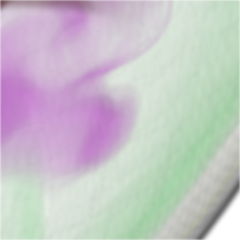
\includegraphics[width=1\textwidth]{../../Neue_Messungen/Supernova/cut/st_ors/st_ors_3.png}
		% \caption*{Quadrat 3 vergrößert dargestellt.}
		% \label{fig::res::sn_comp_st_ors_3}
	\end{minipage}
	\caption{Supernova mit Standard Raycast und variierter Strahlabtastrate berechnet.}
	\label{fig::res::sn_comp_st_ors}
\end{figure}

\begin{figure}[]
	\centering
	\begin{minipage}[t]{0.3\textwidth}
		\centering
		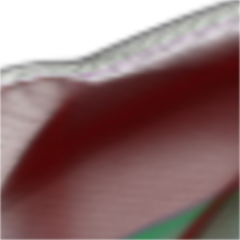
\includegraphics[width=1\textwidth]{../../Neue_Messungen/Supernova/cut/mdc/mdc_1.png}
		% \caption*{Quadrat 1 vergrößert dargestellt.}
		% \label{fig::res::sn_comp_mdc_1}
	\end{minipage}
	\hfill
	\begin{minipage}[t]{0.3\textwidth}
		\centering
		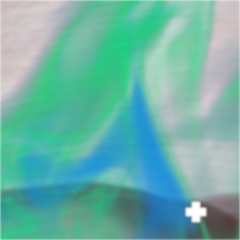
\includegraphics[width=1\textwidth]{../../Neue_Messungen/Supernova/cut/mdc/mdc_2.png}
		% \caption*{Quadrat 2 vergrößert dargestellt.}
		% \label{fig::res::sn_comp_mdc_2}
	\end{minipage}
	\hfill
	\begin{minipage}[t]{0.3\textwidth}
		\centering
		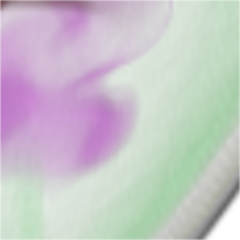
\includegraphics[width=1\textwidth]{../../Neue_Messungen/Supernova/cut/mdc/mdc_3.png}
		% \caption*{Quadrat 3 vergrößert dargestellt.}
		% \label{fig::res::sn_comp_mdc_3}
	\end{minipage}
	\caption{Supernova mit MDC Raycast und ohne variierter Strahlabtastrate berechnet.}
	\label{fig::res::sn_comp_mdc}
\end{figure}

\begin{figure}[]
	\centering
	\begin{minipage}[t]{0.3\textwidth}
		\centering
		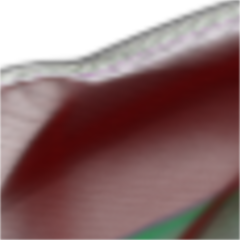
\includegraphics[width=1\textwidth]{../../Neue_Messungen/Supernova/cut/mdc_ors/mdc_ors_1.png}
		% \caption*{Quadrat 1 vergrößert dargestellt.}
		% \label{fig::res::sn_comp_mdc_ors_1}
	\end{minipage}
	\hfill
	\begin{minipage}[t]{0.3\textwidth}
		\centering
		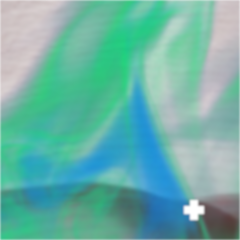
\includegraphics[width=1\textwidth]{../../Neue_Messungen/Supernova/cut/mdc_ors/mdc_ors_2.png}
		% \caption*{Quadrat 2 vergrößert dargestellt.}
		% \label{fig::res::sn_comp_mdc_ors_2}
	\end{minipage}
	\hfill
	\begin{minipage}[t]{0.3\textwidth}
		\centering
		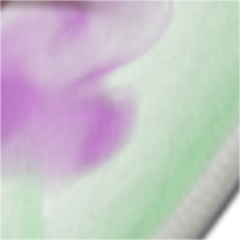
\includegraphics[width=1\textwidth]{../../Neue_Messungen/Supernova/cut/mdc_ors/mdc_ors_3.png}
		% \caption*{Quadrat 3 vergrößert dargestellt.}
		% \label{fig::res::sn_comp_mdc_ors_3}
	\end{minipage}
	\caption{Supernova mit MDC Raycast und variierter Strahlabtastrate berechnet.}
	\label{fig::res::sn_comp_mdc_ors}
\end{figure}

\begin{figure}[]
	\centering
	\begin{minipage}[t]{0.3\textwidth}
		\centering
		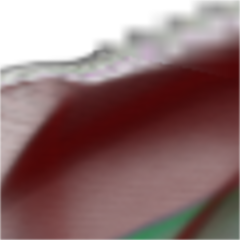
\includegraphics[width=1\textwidth]{../../Neue_Messungen/Supernova/cut/ddc/ddc_1.png}
		% \caption*{Quadrat 1 vergrößert dargestellt.}
		% \label{fig::res::sn_comp_ddc_1}
	\end{minipage}
	\hfill
	\begin{minipage}[t]{0.3\textwidth}
		\centering
		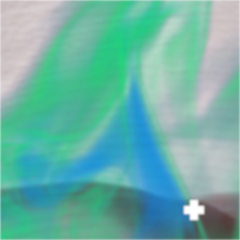
\includegraphics[width=1\textwidth]{../../Neue_Messungen/Supernova/cut/ddc/ddc_2.png}
		% \caption*{Quadrat 2 vergrößert dargestellt.}
		% \label{fig::res::sn_comp_ddc_2}
	\end{minipage}
	\hfill
	\begin{minipage}[t]{0.3\textwidth}
		\centering
		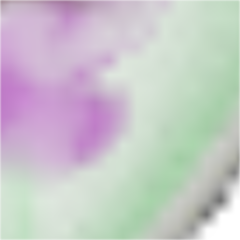
\includegraphics[width=1\textwidth]{../../Neue_Messungen/Supernova/cut/ddc/ddc_3.png}
		% \caption*{Quadrat 3 vergrößert dargestellt.}
		% \label{fig::res::sn_comp_ddc_3}
	\end{minipage}
	\caption{Supernova mit DDC Raycast und ohne variierter Strahlabtastrate berechnet.}
	\label{fig::res::sn_comp_ddc}
\end{figure}

\begin{figure}[]
	\centering
	\begin{minipage}[t]{0.3\textwidth}
		\centering
		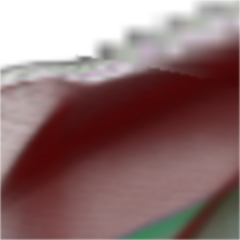
\includegraphics[width=1\textwidth]{../../Neue_Messungen/Supernova/cut/ddc_ors/ddc_ors_1.png}
		% \caption*{Quadrat 1 vergrößert dargestellt.}
		% \label{fig::res::sn_comp_ddc_ors_1}
	\end{minipage}
	\hfill
	\begin{minipage}[t]{0.3\textwidth}
		\centering
		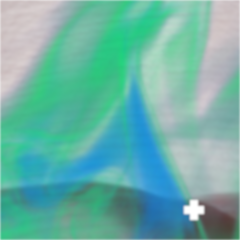
\includegraphics[width=1\textwidth]{../../Neue_Messungen/Supernova/cut/ddc_ors/ddc_ors_2.png}
		% \caption*{Quadrat 2 vergrößert dargestellt.}
		% \label{fig::res::sn_comp_ddc_ors_2}
	\end{minipage}
	\hfill
	\begin{minipage}[t]{0.3\textwidth}
		\centering
		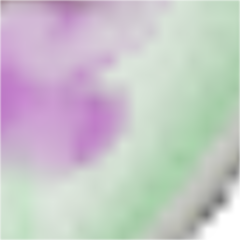
\includegraphics[width=1\textwidth]{../../Neue_Messungen/Supernova/cut/ddc_ors/ddc_ors_3.png}
		% \caption*{Quadrat 3 vergrößert dargestellt.}
		% \label{fig::res::sn_comp_ddc_ors_3}
	\end{minipage}
	\caption{Supernova mit DDC Raycast und ohne variierter Strahlabtastrate berechnet.}
	\label{fig::res::sn_comp_ddc_ors}
\end{figure}

% \clearpage

\subsection{Performanz}
Für die Messung der Performanz der Implementierungen wurden zwei Messwerte bei einer Berechnung eines Bildes genommen.
Die Ausführungszeit des Kernels innerhalb einer Ausführung der \emph{paintGL()}-Methode und die Ausführungszeit der \emph{paintGL()}-Methode selbst.
Dies wurde deshalb so gewählt, da die Implementierungen nicht ausschließlich innerhalb des Kernels durchgeführt wurden, sondern auch außerhalb der Kernelaufrufe Programmcode geschrieben wurde und der Start einer Kernelausführung sowie die synchronisierte Beendigung eine gewisse Zeit brauchen.
Die Ausführungszeit der \emph{paintGL()}-Methode ist letztendlich der Wert, welcher die reale spürbare Performanz für den Nutzer angibt.

Für die Messungen der Performanz wurde kein Eyetracking verwendet, da dies lediglich die Mausposition mit der Blickposition ersetzt und keinen Einfluss auf die Ausführungszeit des Kernels und nur einen konstanten Einfluss auf die Ausführungszeit der \emph{paintGL()}-Methode hat.
Auch sollten, bei den Messungen mit den verschiedenen Methoden, möglichst die selben Mauspositionen verwendet werden, um vergleichbare Ergebnisse zu erhalten.
Die Verwendung eines Eyetrackers würde es fast unmöglich machen, die selben Blickpunkte in einem gewissen Zeitraum zu fokussieren.

Für die Messergebnisse selbst wurde ein spiegelverkehrtes \emph{S} mit dem Mauszeiger auf einem Bild nachgefahren und dabei die Mauspositionen abgespeichert.
Insgesamt wurden hier 584 Mauspositionen aufgezeichnet.
Es wurden anschließend verschiedene Volumendaten mit jeweils drei verschiedenen Transferfunktionen für die drei verschiedenen Implementierungen, den Standard-, \emph{MDC}- und \emph{DDC}-Raycast sowie jeweils einmal mit konstanter und einmal mit variierter Strahlabtastrate für die Messungen verwendet.
Bei jeder dieser Messung wurde dabei für jede der Mauspositionen des gespeicherten Mausverlaufs ein Bild berechnet und zu dieser Berechnung die Mausposition, die Ausführungszeit des Kernels und die Ausführungszeit der \emph{paintGL()}-Methode gespeichert.

Die Hardware des Computers, mit welchem die Messungen durchgeführt wurden, besteht unter Anderem aus einem \emph{Intel Core i5 4670k bei $3,40$\,GHz} CPU und einer \emph{GIGABYTE AMD Radeon (TM) R9 390 Series} GPU.
Die Auflösung der zu berechnenden Bilder betrug immer $2263\times1306$\,Pixel.

Die Messungen wurden mit den Volumen \emph{Bonsai}, \emph{Supernova} und \emph{Chameleon} durchgeführt.
Das Volumen \emph{Bonsai} hat eine Auflösung von $256\times256\times256$\,Voxel, wobei die Voxel eine Slice-Dicke von $1,0\times1,0\times1,0$ haben.
Das Volumen \emph{Supernova} hat eine Auflösung von $432\times432\times432$\,Voxel, wobei die Voxel eine Slice-Dicke von $1,0\times1,0\times1,0$ haben.
Das Volumen \emph{Chameleon} hat eine Auflösung von $1024\times1024\times1024$\,Voxel, wobei die Voxel eine Slice-Dicke von $0,09228515625\times0,09228515625\times0,105$ haben.

\begin{figure}
	\centering
	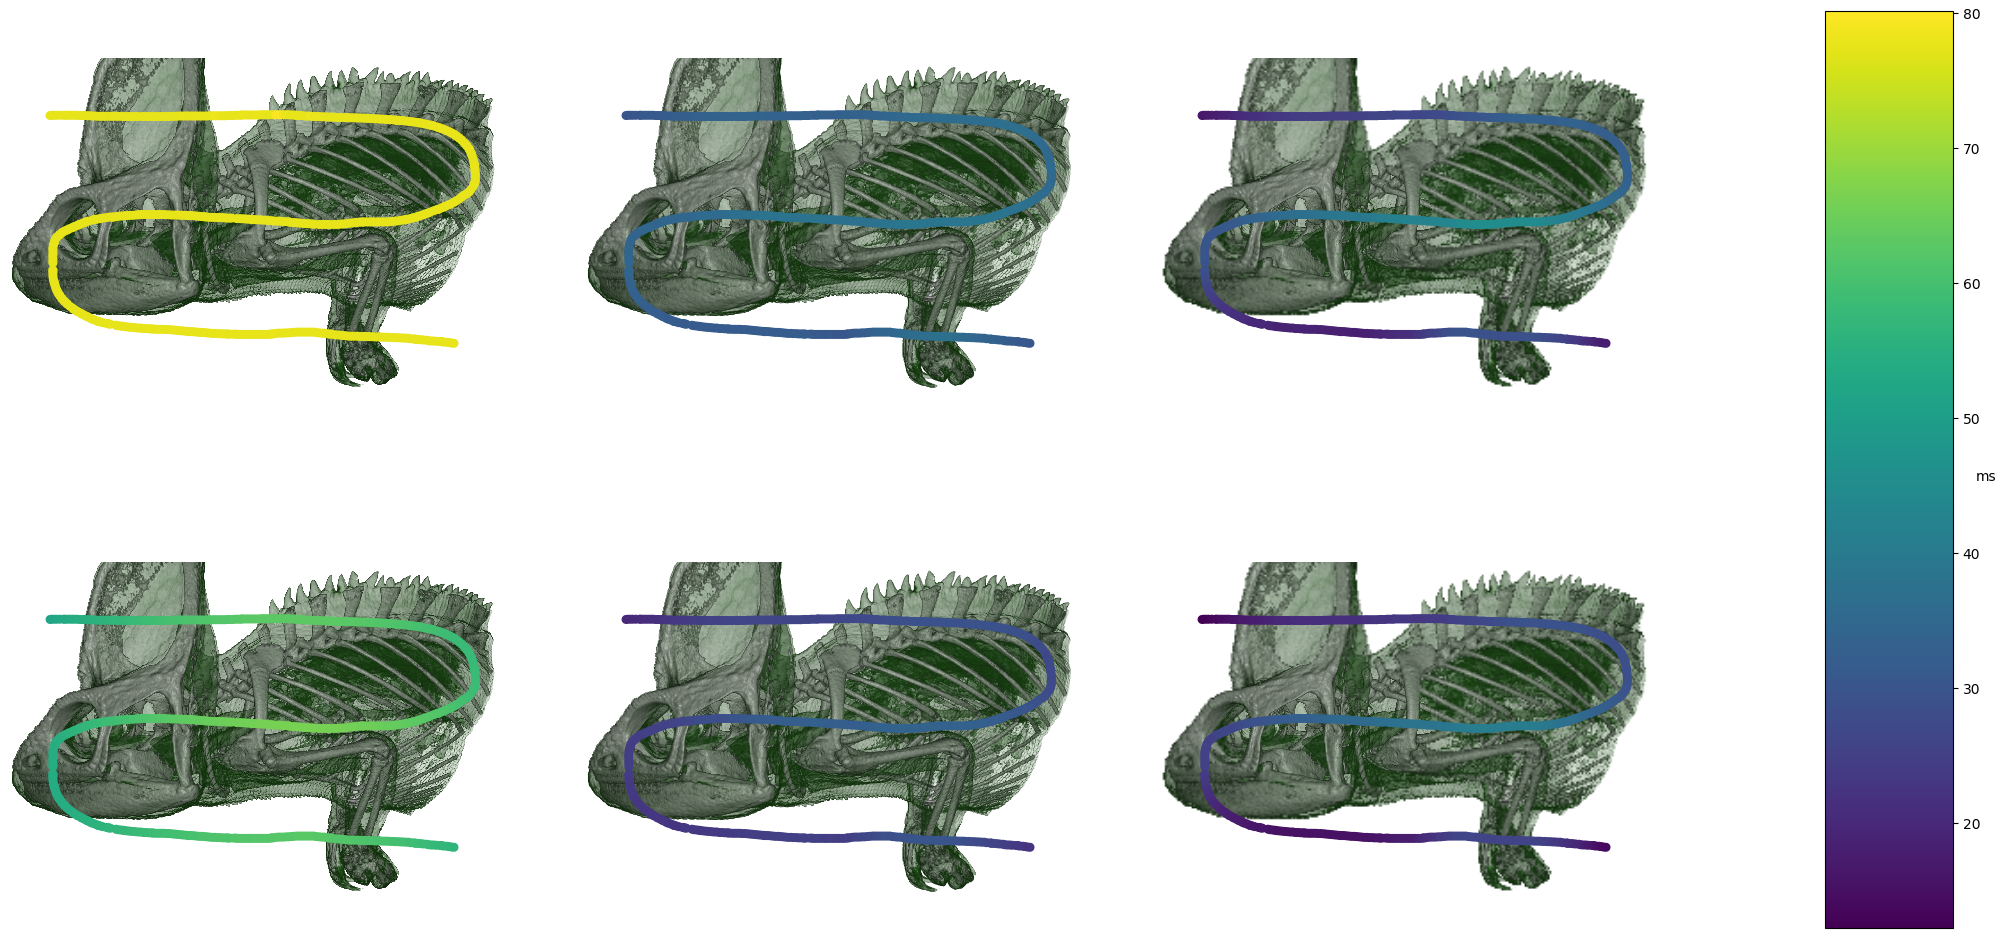
\includegraphics[width=1\textwidth]{../../Neue_Messungen/Chameleon/heatmaps/hm_wa.png}
	\caption{Heatmaps der verschiedenen Verfahren für das Volumen Chameleon. Für verschiedene Mauspositionen wurde eine Berechnung durchgeführt. Die jeweilige Ausführungszeit des Kernels für diese Berechnung wurde entsprechend des Farbbalkens farblich eingezeichnet. Der Farbbalken gibt die Werte in \,ms an. \emph{v. S. a. r.} steht für \emph{variierter Strahlabtastrate}}
	\label{fig::res::pf::hm_wa}
\end{figure}

Für einen anschaulichen Vergleich der Methoden wurde für die Messungen des Volumen Chameleon Heatmaps erstellt (Abbildung \ref{fig::res::pf::hm_wa}).
Die gemessene Ausführungszeiten des Kernels für die unterschiedlichen Mauspositionen wurden für die Erstellung der Heatmaps verwendet.
Da die Differenz zwischen Ausführungszeit des Kernels und der Ausführungszeit der \emph{paintGL()}-Methode unabhängig von dem zu berechnenden Volumen und der verwendeten Transferfunktion ist, wurde diese hier nicht einbezogen.

Abbildung \ref{fig::res::pf::hm_wa} zeigt, dass die Ausführungszeit des Kernels für den Standard Raycast ohne variierter Strahlabtastrate für alle Mauspositionen im Bereich von 80\,ms liegt und damit im Vergleich zu den anderen Methoden am höchsten ist.
Betrachtet man nun die Standard Variante mit variierter Strahlabtastrate, so kann man eine allgemeine Verbesserung feststellen.
Die Ausführungszeit des Kernels liegt bei dieser Methode bei circa 65\,ms und variiert je nach Mausposition leicht.
So ist die Ausführungszeit für eine Mausposition am oberen und unterem Rande des Bildes ein wenig geringer, als wenn diese sich in der Mitte des Bildes befindet.
Die Heatmap zur Methode mit dem MDC Raycast und ohne variierter Strahlabtastrate zeigt zu beiden Standard Raycast Methoden eine Verbesserung.
Die Ausführungszeit des Kernels liegt hier bei circa 40\,ms und ist im mittleren Bereich des Bildes minimal höher als im oberen oder unteren Bereich.
Wird der MDC Raycast mit einer variierten Strahlabtastrate kombiniert, so ist die Ausführungszeit des Kernels im oberen und unteren Bereich des Bildes sichtbar schneller, als in der Variante ohne einer variierten Strahlabtastrate.
Im mittleren Bereich des Bildes liegt sie nun bei circa 35\,ms und in den äußeren Bereichen des Bildes liegt sie bei circa 20\,ms.
Die Heatmap zum DDC Raycast zeigt, dass mit dem DDC Raycast je nach Mausposition die niedrigsten Ausführungszeit des Kernels erreicht wurde.
Auch ohne einer variierten Strahlabtastrate zeigt der DDC Raycast verhältnismäßig ein ähnliches Muster, wie der Standard und MDC Raycast mit variierter Strahlabtastrate.
Die Ausführungszeit des Kernels betrug hier im äußeren Bild ebenfalls geringere Werte als im mittigen Bereich des Bildes.
Im äußeren Bereich betrug sie circa 20\,ms und im mittleren circa 45\,ms.
Es ist auffallend, dass die Differenz zwischen der Ausführungszeit des Kernels im oberen und unteren Bereich und der Ausführungszeit im mittleren Bereich des Bildes hier größer als bei den anderen Verfahren ist.
In der Heatmap zum DDC Raycast mit variierter Strahlabtastrate ist zu erkennen, dass die äußeren Bereiche des Bildes, besonders oben links und unten rechts, nochmal niedrigere Ausführungszeiten des haben, als im DDC Raycast ohne variierter Strahlabtastrate.
In den äußeren Bereichen fällt diese auf bis zu 15\,ms und im mittleren Bereich auf leicht über 40\,ms.
Vergleicht man die Heatmaps des DDC und MDC Raycasts miteinander, so fällt auf, dass der DDC Raycast in den äußeren Bereichen des Bildes niedrigere Ausführungszeiten als der MDC Raycast erreicht, dafür die Ausführungszeiten des DDC Raycasts im mittleren Bereich des Bildes leicht höher ist, als die des MDC Raycasts.

Das die Ausführungszeiten im äußeren Bereich des Bildes geringer sind wird zwei unterschiedliche Gründe haben.
Erstens wird, wenn sich die Mausposition weiter weg von dem Volumen befindet, ein Großteil des Volumens beziehungsweise des Bildes mit einer geringeren Strahlabtastrate abgetastet, wodurch und einige Work-Items und Work-Groups früher terminieren können.
Zweitens ist die Bildabtastrate in der Nähe der Mausposition am höchsten.
Ist diese am Rande des Volumens, wie es in Abbildung \ref{fig::res::pf::hm_wa} auch der Fall ist, so fällt ein großer Anteil der Strahlen auf Bereiche, in denen nur wenige Voxel abgetastet werden müssen und dadurch wieder einige Work-Items und Work-Groups früher terminieren.
Das die MDC Methode ohne einer variierten Strahlabtastrate auch in den äußeren Bereichen eine relativ gleiche Ausführungszeit hat, wie in den inneren Bereichen des Volumens, wird daran liegen, dass der hoch aufgelöste innere Bereich des MDC Raycasts deutlich kompakter und ein wenig kleiner ist, als der des DDC Raycasts.
Dadurch fallen auch weniger Strahlen des hoch aufgelösten Bereichs außerhalb des Volumens, auch wenn sich die Mausposition am Rande des Volumens befindet.

\begin{figure}
	\centering
	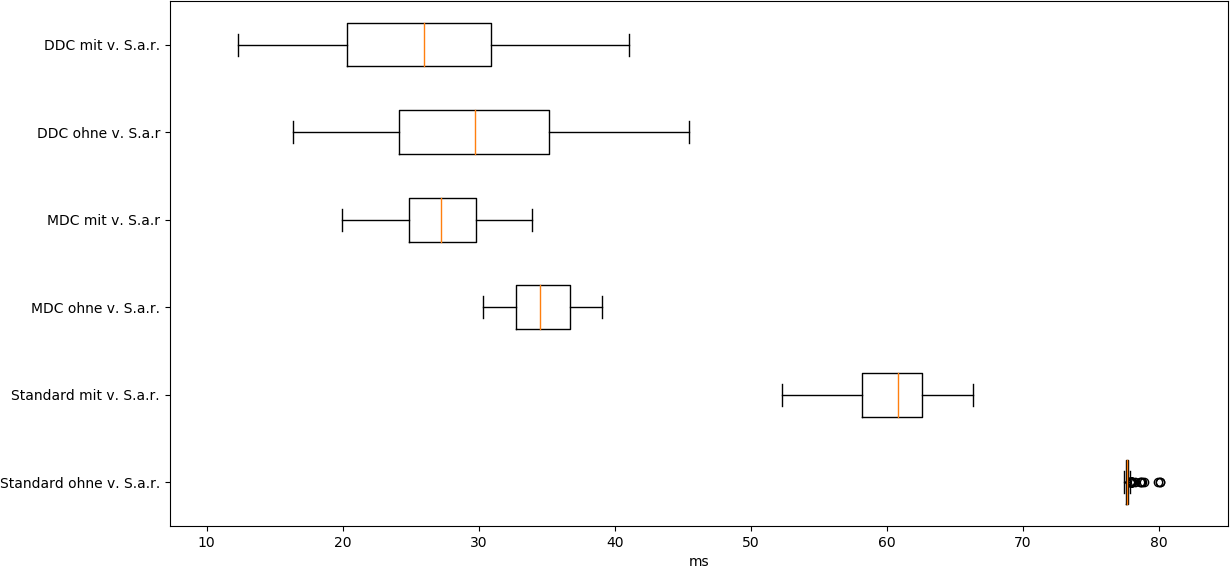
\includegraphics[width=1\textwidth]{../../Neue_Messungen/Chameleon/boxplots.png}
	\caption{Boxplots der Ausführungszeiten des Kernels der verschiedenen Verfahren bei der Verwendung des Volumen Chameleon. Die Box reicht von den unteren Viertel bis zu den oberen Viertel der Werte und der Median ist orange eingezeichnet.}
	\label{fig::res::pf::bp}
\end{figure}

Die Ausführungszeiten des Kernels der unterschiedlichen Methoden, wie sie in den Heatmaps (Abbildung \ref{fig::res::pf::hm_wa}) farbig dargestellt wurden, sind in Abbildung \ref{fig::res::pf::bp} als Boxplots dargestellt.
Wie an den Heatmaps schon ersichtlich war, sind die Ausführungszeiten des Standard Raycast ohne variierter Strahlabtastrate am höchsten und relativ gleich.
Die Messwerte sind konzentriert um die 77,5\,ms.
Die Ausführungszeiten für den Standard Raycast mit variierter Strahlabtastrate sind ein wenig geringer und sind untereinander stärker verteilt.
Für den MDC Raycast sieht es ähnlich aus.
Ohne variierter Strahlabtastrate sind die Werte ein wenig höher und dafür kompakter.
Mit einer variierten Strahlabtastrate sind sind die Werte niedriger aber weiter verteilt.
Anders wie bei den vorherigen Raycast Methoden sind die Ausführungszeiten des DDC Raycast mit variierter Strahlabtastrate ein wenig kopakter, als ohne variierter Strahlabtastrate.
Mit variierter Strahlabtastrate sind die Werte insgesamt aber trotzdem niedriger.

\begin{figure}
	\centering
	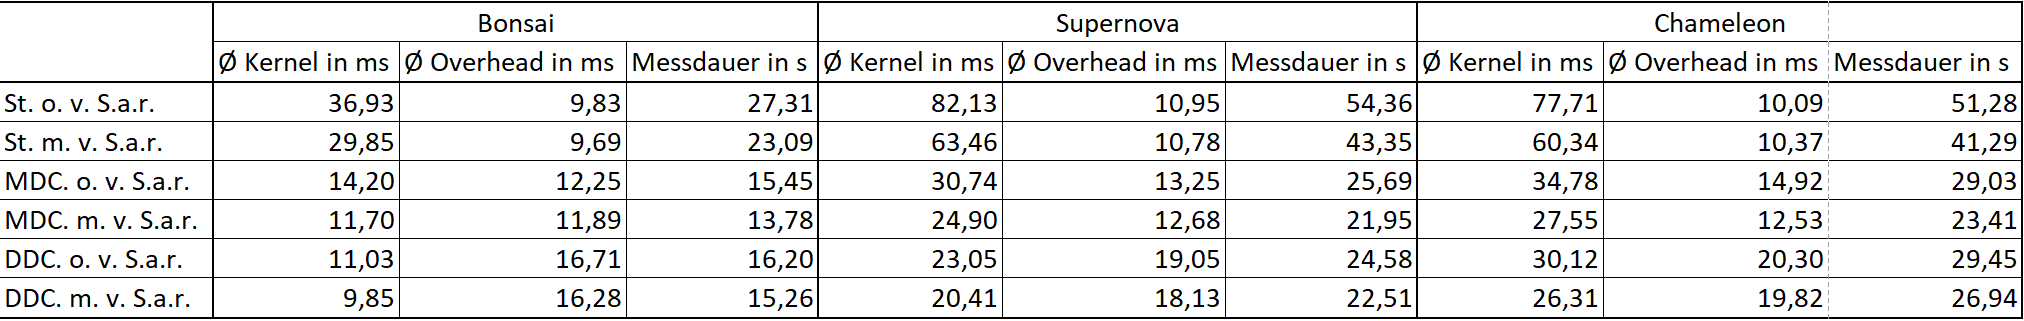
\includegraphics[width=1\textwidth]{../../Neue_Messungen/Messungen_in_Tabelle.PNG}
	\caption{Die Ergebnisse der verschiedenen Verfahren mit den Volumen Bonsai, Supernova und Chameleon. Für jedes Verfahren und Volumen ist die durchschnittliche Ausführungszeit des Kernel (K.) und die Varianz von dieser sowie der durchschnittliche Overhead (Oh.) und die summierte Ausführungszeit der \emph{paintGL()}-Methode (Md.) für die verschiedenen Mauspositionen angegeben.}
	\label{fig::res::pf::table}
\end{figure}

Wie schon in Abbildung \ref{fig::res::pf::hm_wa} und \ref{fig::res::pf::bp} die Verhältnisse der Ausführungszeiten der verschiedenen Methoden dargestellt wurden, wird dies in Abbildung \ref{fig::res::pf::table} durch die genauen Werte bestätigt.
In Abbildung \ref{fig::res::pf::table} sind für die unterschiedlichen Verfahren und die Volumen Bonsai, Supernova und Chameleon die durchschnittliche Kernelzeit, dessen Varianz sowie der durchschnittliche Overhead der \emph{paintGL()}-Methode ohne die Ausführungszeit des Kernels dargestellt.
Zusätzlich ist auch die summierte Ausführungszeit der \emph{paintGL()}-Methode für die insgesamt 584 verschiedenen Berechnungen jeder Messung angegeben.

Betrachtet man den Overhead der verschiedenen Methoden, so sieht man, dass der Standard Raycast für die unterschiedlichen Volumen ähnlich ist und mit circa 10\,s den geringsten Overhead hat.
Die Implementierung des Standard Raycasts verwendet auch nur einen Kernel Aufruf.
Der Overhead des MDC Raycasts ist ein wenig höher als der des Standard Raycasts und beträgt für das Bonsai Volumen circa 12\,s, für das Supernova Volumen circa 13\,s und für das Chameleon Volumen circa 14\,s.
Der Overhead des DDC Raycasts ist am höchsten und beträgt für den Bonsai circa 16\,s, für die Supernova circa 19\,s und für das Chameleon circa 20\,s.
Sowohl der MDC Raycast als auch der DDC Raycast verwenden jeweils zwei Kernel Aufrufe aber der DDC Raycast berechnet vor der Ausführung des Kernels noch einige Werte, die für diesen Raycast benötigt werden.

Vergleicht man die verschiedenen Volumen, so wird das Bonsai Volumen deutlich schneller als das Supernova oder Chameleon Volumen berechnet.
Dies wird hauptsächlich an der geringeren Auflösung des Volumens und damit einer deutlich geringeren Anzahl an Voxeln liegen.
Im Widerspruch dazu benötigt aber die Messung für das Supernova Volumens etwas länger, als die Messung für das Chameleon Volumen.
Die Wahl der Transferfunktion in Verbindung mit dem in allen Raycasts vorimplementierten \emph{Empty-Space-Skipping (ESS)} könnte hier eine Rolle spielen.
Werden in einem Volumen die Voxel nicht vollständig transparent gemacht, sondern haben immer noch einen gewissen Opazitätswert, so werden diese nicht durch das ESS übersprungen, was zu einer längeren Berechnung führt.
Ein weiterer Grund ist kann die Perspektive auf die Volumen sein.
Das Chameleon Volumen wird von der Seite betrachtet und hat aufgrund der nicht einheitlichen Slice-Dicken eine geringere Tiefe, wenn man es von der Seite betrachtet.
Daher terminieren die Strahlen von der Seite früher.
Das Supernova Volumen hingegen ist relativ rund und hat eine einheitlich Slice-Dicke.

\section{Diskussion}\label{sec::disc}
% Bildqualität: Abstrakter, was sieht gut, was eher schlechter aus. Einfluss der variierten Bild- und Strahlabtastrate.
% Performanz: Nochmal das Standard am langsamsten ist, mit v. Sar. aber beschleunigt. DDC die schnellsten Werte erreicht aber MDC insgesmat schneller und geringere varianz, dadurch fühlt es sich weicher an, da ddc ruckler hat
% Verknüpfung mit Eyetracker
% Tradeoff Bildqualität MDC DDC Standard, MDC insgesamt am besten
% Transferfunktion parameter, Interpolationparameter
% DDC optimierbar
Betrachtet man rückblickend auf die Ergebnisse die unterschiedlichen Bildabtastraten, so ist es offensichtlich, dass der Standard Raycast von den unterschieldichen Methoden her, die beste Bildqualität erzeugt.
Trotzdem kann durch das Ausnutzen der Limitierungen des visuellen Wahrnehmungssystems des Menschen bei der Verwendung eines Eyetrackers annähernd der Effekt erzeugt werden, dass die Raycast Methoden MDC und DDC das Bild in voller Auflösung berechnen, obwohl dies nicht der Fall.
Da die Auflösung beim MDC Raycast im äußeren Bereich im Vergleich zum DDC Raycast immer noch deutlich höher ist, ist dieser Effekt für den MDC Raycast viel realistischer und kaum wahrnehmbar während beim DDC Raycast noch Artefakte des am niedrigsten aufgelösten Bereichs wahrnehmbar sind.
Um die Bildqualität des DDC Raycasts weiter zu verbessern, könnte die Bildabtastrate des äußersten Bereichs angehoben und oder der Radius des mittleren Bereichs vergrößert werden, so dass die reduzierte Auflösung noch weniger auffällt.
Für den MDC Raycast hingegen wäre es denkbar, die Auflösung des äußeren Bereichs selbst weiter zu verringern oder einen zusätzlichen Bereich einzufügen, der nur noch ein Achtel der maximalen Auflösung hat.

Betrachtet man rückblickend auf die Ergebnisse die unterschiedlichen Varianten, mit variierter und ohne variierter Strahlabtastrate, so gibt es hier bei den Bildern kaum wahrnehmbare Unterschiede.
Im Gegensatz zu den statischen Bildern wurde aber bei aktivem Eyetracking bei den Varianten mit variierter Strahabtastrate, Artefakte durch die veränderte Strahlabtastrate im Bild wahrgenommen, wenn sich die Augen über das Bild bewegt haben.
Während einer Fixation verblassen diese Artefakte und sind wie bei einem statischen Bild kaum mehr wahrnehmbar.
Die Ergebnisse scheinen anzudeuten, dass die Strahlabtastrate im äußeren Bereich noch weiter reduziert werden könnte, da diese bisher nur auf ein Minimum von ein Viertel der normalen Strahlabtastrate nach außen hin fallen kann.
In weiteren Tests hat das Reduzieren des Limits auf ein Fünftel schon deutlich Artefakte der Unterabtastung ergeben, die dafür aber auch nur an den vom Blickpunkt entferntesten Stellen aufgetreten sind und daher nicht so aufgefallen sind.
Weiter wäre es denkbar, die Funktion, die die Strahlabtastrate abhängig von der Distanz zur Mausposition anpasst, abzuändern, so dass diese schon bei einer geringeren Entfernung stärker abnimmt und früher das Limit erreicht.
Da selbst bei nur einem Viertel der maximalen Strahlabtastrate im äußeren Bereich kaum Artefakte wahrnehmbar sind, sollte dies ohne eine wahrnehmbare Reduzierung der Bildqualität möglich sein.

Hinsichtlich der Ausführungszeit des Kernels zeigen die Ergebnisse deutlich, dass der Standard Raycast ohne variierter Strahlabtastrate am schlechtesten abschneidet.
Der MDC Raycast ohne variierter Strahlabtastrate ist hier besser und hat aber eine höhere Varianz.
Der DDC Raycast ebenfalls ohne variierter Strahlabtastrate erreicht deutlich geringere Kernelausführungszeiten als der MDC Raycast und hat einen niedrigeren Median und Durchschnitt.
Dafür erreicht der DDC Raycast im Vergleich zum MDC Raycast aber auch deutlich höhere Kernelausführungszeiten und hat daher auch eine deutlich höhere Varianz.
Wird zusätzlich zu den verschiedenen Methoden eine variierte Strahlabtastrate verwendet, so verringert sich bei allen Methoden die Kernelausführungszeiten und bis auf den DDC Raycast, bei dem sich die Varianz dadurch ein wenig verringert hat, hat sich beim Standard und MDC Raycast die Varianz dadurch erhöht.

Hinsichtlich der wahrgenommenen Performanz, also der Ausführungszeiten inklusive des Overheads, schneidet der MDC Raycast trotz einer höheren durchschnittlichen Kernelausführungszeit aufgrund des geringeren Overheads besser ab, als der DDC Raycast.
Da zusätzlich die Varianz des MDC Raycasts geringer ist und dies daher auch bei der Verwendung eines Eyetrackers zu weniger Verzögerungen führt, als beim DDC Raycasts sowie der MDC Raycast bei Mauspositionen, die sich innerhalb des Volumens befinden, sich besser verhält, ist aus Sicht der Performanz der MDC Raycast mit variierter Strahlabtastrate die beste Wahl.
Da zusätzlich der MDC Raycast höherwertige Bilder als der DDC Raycast generiert, trotzdem der Verlust der Bildqualität bei der Verwendung eines Eyetrackers im Vergleich zum Standard Raycast nicht wahrnehmbar ist, schneidet der MDC Raycast mit variierter Strahlabtastrate in Verbindung mit einem Eyetracker von den verschiedenen Methoden her insgesamt am besten ab.

Dass der MDC Raycast von der Performanz her besser abschneidet als der DDC Raycast liegt an unterschiedlichen Faktoren.
So ist wie genannt, der Overhead ein wichtiger Faktor, der die wahrnehmbare Performanz des DDC Raycasts im Vergleich zum MDC Raycast beeinträchtigt.
Ein weiterer Faktor ist die Umsetzung des Index-Mappings.
Aufgrund dessen, dass dieses versucht wurde variabel zu halten, wurden viele Berechnungen für das Abbilden der Indizes durchgeführt, bevor der eigentliche Raycast beginnt.
Die Work-Items werden hier anhand ihrer globalen ID auf völlig unterschiedliche Bildkoordinaten abgebildet.
Dies passiert unabhängig davon, in welcher Work-Group sie sich befinden, wodurch unter Umständen sehr unterschiedliche Bereiche durch eine Work-Group berechnet werden und die gesamte Work-Group immer auf das langsamste Work-Item warten muss.
Eine Änderung der Implementierung dahingehend, dass die Work-Items nicht anhand der globalen ID sondern anhand der Work-Group ID mit der gesamten Work-Group auf einen zusammen liegenden Block von Bildkoordinaten abgebildet werden, würde die Ausführungszeit vieler Work-Groups verbessern.
Ein anderer Faktor ist die Art und Weise, wie die NDRange des Kernels festgelegt wird.
Eine Anpassung dieser, dass sie in mindestens eine Dimension ein Vielfaches der Work-Group Größe ist, würde die Anzahl zu startender Work-Groups reduzieren und die Ausführungszeit des Kernels weiter verbessern.
Die hohe Varianz des DDC Raycasts liegt vermutlich also vor allem an der Art der Implementierung.
Eine Optimierung dieser Implementierung würde sowohl die Ausführungszeit des Kernels, als auch den Overhead reduzieren, so dass der DDC Raycast insgesamt eine bessere Performanz als der MDC Raycast hat.